\documentclass[12pt]{article}

\pdfoutput=24
\usepackage{amsmath}
\usepackage{amsthm}
\usepackage{esvect}
\usepackage[toc,page]{appendix}
\usepackage{leftidx}
\usepackage{color}
\usepackage{framed, color}
\usepackage{multirow}
\usepackage{pdfpages}
\usepackage{multicol}
\usepackage{wrapfig,lipsum,booktabs}
\usepackage[font=small,skip=0pt]{caption}

\usepackage[utf8]{inputenc}
\usepackage{mathtools,hyperref}
\hypersetup{
    colorlinks=true,
    linkcolor=cyan,
    filecolor=cyan,      
    urlcolor=red,
    citecolor=red,
}

\usepackage{cleveref}
\usepackage{commath}
\usepackage{enumitem}
\usepackage{amssymb}
\renewcommand{\qedsymbol}{$\blacksquare$}

%%%%%%%%%%%
%%%%%%%%%%%  User Defined Commands. (macros)
%%%%%%%%%%%

\definecolor{mgreen}{RGB}{25,147,100}
\definecolor{shadecolor}{rgb}{1,.8,.1}
\definecolor{shadecolor2}{RGB}{245,237,0}
\definecolor{orange}{RGB}{255,137,20}
\definecolor{orange}{RGB}{245,37,100}

%%%%%%%%%%%
%%%%%%%%%%%  Graphical Packages
%%%%%%%%%%%
\usepackage{pgfplots}
\usetikzlibrary{patterns}
\usepackage{mdframed}
\usepackage{adjustbox}
\usepackage{tcolorbox}
%\usepackage{graphics}
\usepackage{tikz,ifthen,fp,calc}
\usepackage{caption}
\usepackage{subcaption}
\usetikzlibrary{plotmarks}
\usepackage{graphicx}

%%%%%%%%%%%%%%%%%
%%%%%%%%%%%%%%%%% Theorem Styles
%%%%%%%%%%%%%%%%%
\theoremstyle{plain}
\newtheorem{theorem}{Theorem}[section]
\newtheorem{prop}{Proposition}[section]
\newtheorem{corr}{Corollary}[section]
\theoremstyle{definition}
\newtheorem{definition}{Definition}[section]
\newtheorem{lemma}[theorem]{Lemma}
\theoremstyle{definition}
\newtheorem{remark}{Remark}[section]
\newtheorem{fact}{Fact}[section]

\usepackage[english]{babel}
\usepackage{babel,blindtext}
\newtheorem{corollary}{Corollary}[theorem]
\newtheorem{exmp}{Example}[section]
\usepackage{fullpage}
\usepackage{amsfonts}
\usepackage{lscape}
\usepackage{bbm}

\usepackage{todonotes}
\usepackage{cite}
\usepackage{verbatim}
\usepackage{bm}

\DeclareMathOperator*{\argmax}{arg\,max}
\usepackage[margin=1in]{geometry}
\providecommand{\keywords}[1]{\textbf{\textit{Keywords:---}} #1}

\usepackage[T1]{fontenc}
\usepackage[utf8]{inputenc}
\usepackage{authblk}
\usepackage{cite}


\newcommand*{\affaddr}[1]{#1} % No op here. Customize it for different styles.
\newcommand*{\affmark}[1][*]{\textsuperscript{#1}}
%\newcommand*{\email}[1]{\texttt{#1}}

\title{\textbf{Codling Moth}}

\author[1]{Kirti Rajagopalan \thanks{kirtir@wsu.edu}}
\affil[1]{CAHNR, Washington State University}

\date{}

\providecommand{\keywords}[1]{\textbf{\textit{Keywords:}} #1}

\begin{document} 

\maketitle

\begin{abstract}
  Abstract Goes Here
\end{abstract}


\keywords{Codling Moth, pest, pesticide, pest management}

\section{Introduction}

Limited work characterizing the impacts of climate change on insects.
Touch upon shifts that have already been observed based on historical records as well (see references).
Higher pest pressure is widely noted as a potential climate change risk to food production  and pests are a particular concern for specialty crops for which product quality is paramount.
Across the globe, shifts in the ranges of insect pests have been documented in response to climate changes~\cite{Bebber_2013, Parmesan_Camille, Jaramillo_2009}, though some~\cite{Battisti_Andrea} have argued that there is in fact a surprising paucity of documented examples, raising the possibility that trophic interactions or other mechanisms may make insect pests less sensitive to direct climate effects than previously thought.

Washington State in an economically important apple production area, representing 66\% of US apple production (USDA NASS 2018) (making it PNW only raises this to $68\%$; WA also represents 43\% of the pear production but not sure if that’s relevant here). Apples are the leading commodity in Washington State, accounting for \$2.4 billion in 2016, 22\% of the total value of agricultural production (USDA NASS 2017).
	Importance of controlling the codling moth for the tree fruit industry. Some industry statistics

Our objective.

\section{Background(Kirti, Georgine)}


\subsection{Study Area (Georgine)}


\subsection{Codling moth life cycle (Sonia, Ute)}


\subsection{Codling moth management (Ute)}


\subsection{Climate and climate change impacts on pests(Georgine/Sonia)}


We need a thorough literature review for pests in general 
and codling moth in particular. Looks like it is most related to aphids. 
Temperature has a strong and direct influence on insect 
development, reproduction and survival~\cite{Bale2002_451},
and climate is thus expected to directly impact insect pests 
through effects on their ranges~\cite{Jaramillo_2009, Estay_01380}, 
winter mortality (citation), development timing (citation needed), 
voltinism (the number of annual generations) \cite{Altermatt_Florian}(Leudling et al. 2011), 
and the duration of the reproductive period~\cite{van_Asch}. 
Indirect effects are also possible, including effects on natural enemies, 
competitors, or responses to climate-induced changes on the host plant 
\cite{Bale2002_451, Gregory_2009}. The IPCC has concluded that 
work to date projecting likely climate impacts has suggested a tendency 
for risk of insect damage to agricultural plants to increase, though but 
also notes that current scenario analyses of pests are typically limited 
by simplistic assumptions, and it remains to be seen how conclusions 
may change when scenarios incorporate more sophisticated factors such 
as migration and invasion patterns and other types of global change 
(Porter et al. 2014).
A number of different researchers have examined the potential 
impacts of climate change on codling moth in different areas of 
the world, including in Norway~\cite{Rafoss_Trond}, eastern 
Washington~\cite{Nelson_higgins}, California (Leudling et al. 2011), 
Switzerland~\cite{Stoeckli_2012}, and Poland~\cite{Juszczak2013}.  
In general, studies have suggested an advancement in key 
phenological stages, and a concomitant increase in the 
number of generations per season. This in turn suggests 
a need for control measures over a longer time period in 
the future, with negative economic implications and higher 
risk for the development of resistance.

Can we add something related to gaps. That is what are we offering beyond rehashing what is out there?

\section{Methods}
%%%%%%%%%%%%%%%%%%%%%%%%%%%%%%%%%%%%%%%%%%%%%%%%%
%%%%%%%%%%%%%%%%%%%%%%%%%%%%%%%%%%%%%%%%%%%%%%%%%
\subsection{Input data  (Sonia)}
%%%%%%%%%%%%%%%%%%%%%%%%%%%%%%%%%%%%%%%%%%%%%%%%%
%%%%%%%%%%%%%%%%%%%%%%%%%%%%%%%%%%%%%%%%%%%%%%%%%
\subsection{Codling moth degree day model (Vince)}
%%%%%%%%%%%%%%%%%%%%%%%%%%%%%%%%%%%%%%%%%%%%%%%%%
%%%%%%%%%%%%%%%%%%%%%%%%%%%%%%%%%%%%%%%%%%%%%%%%%
\subsection{Diapause induction assumptions (Ute)}
%%%%%%%%%%%%%%%%%%%%%%%%%%%%%%%%%%%%%%%%%%%%%%%%%
%%%%%%%%%%%%%%%%%%%%%%%%%%%%%%%%%%%%%%%%%%%%%%%%%
\subsection{Model application framework (Ute)}

Also discuss distinction between warmer and  colder areas (Giridhar)

%%%%%%%%%%%%%%%%%%%%%%%%%%%%%%%%%%%%%%%%%%%%%%%%%
%%%%%%%%%%%%%%%%%%%%%%%%%%%%%%%%%%%%%%%%%%%%%%%%%
\section{Results (Hossein, Giridhar)}
%%%%%%%%%%%%%%%%%%%%%%%%%%%%%%%%%%%%%%%%%%%%%%%%%
%%%%%%%%%%%%%%%%%%%%%%%%%%%%%%%%%%%%%%%%%%%%%%%%%
\subsection{Changes in degree day accumulation (Min to help Hossein)}
Show annual and seasonal changes

\begin{figure}[h!]
\begin{subfigure}{.46\textwidth}
  \centering
  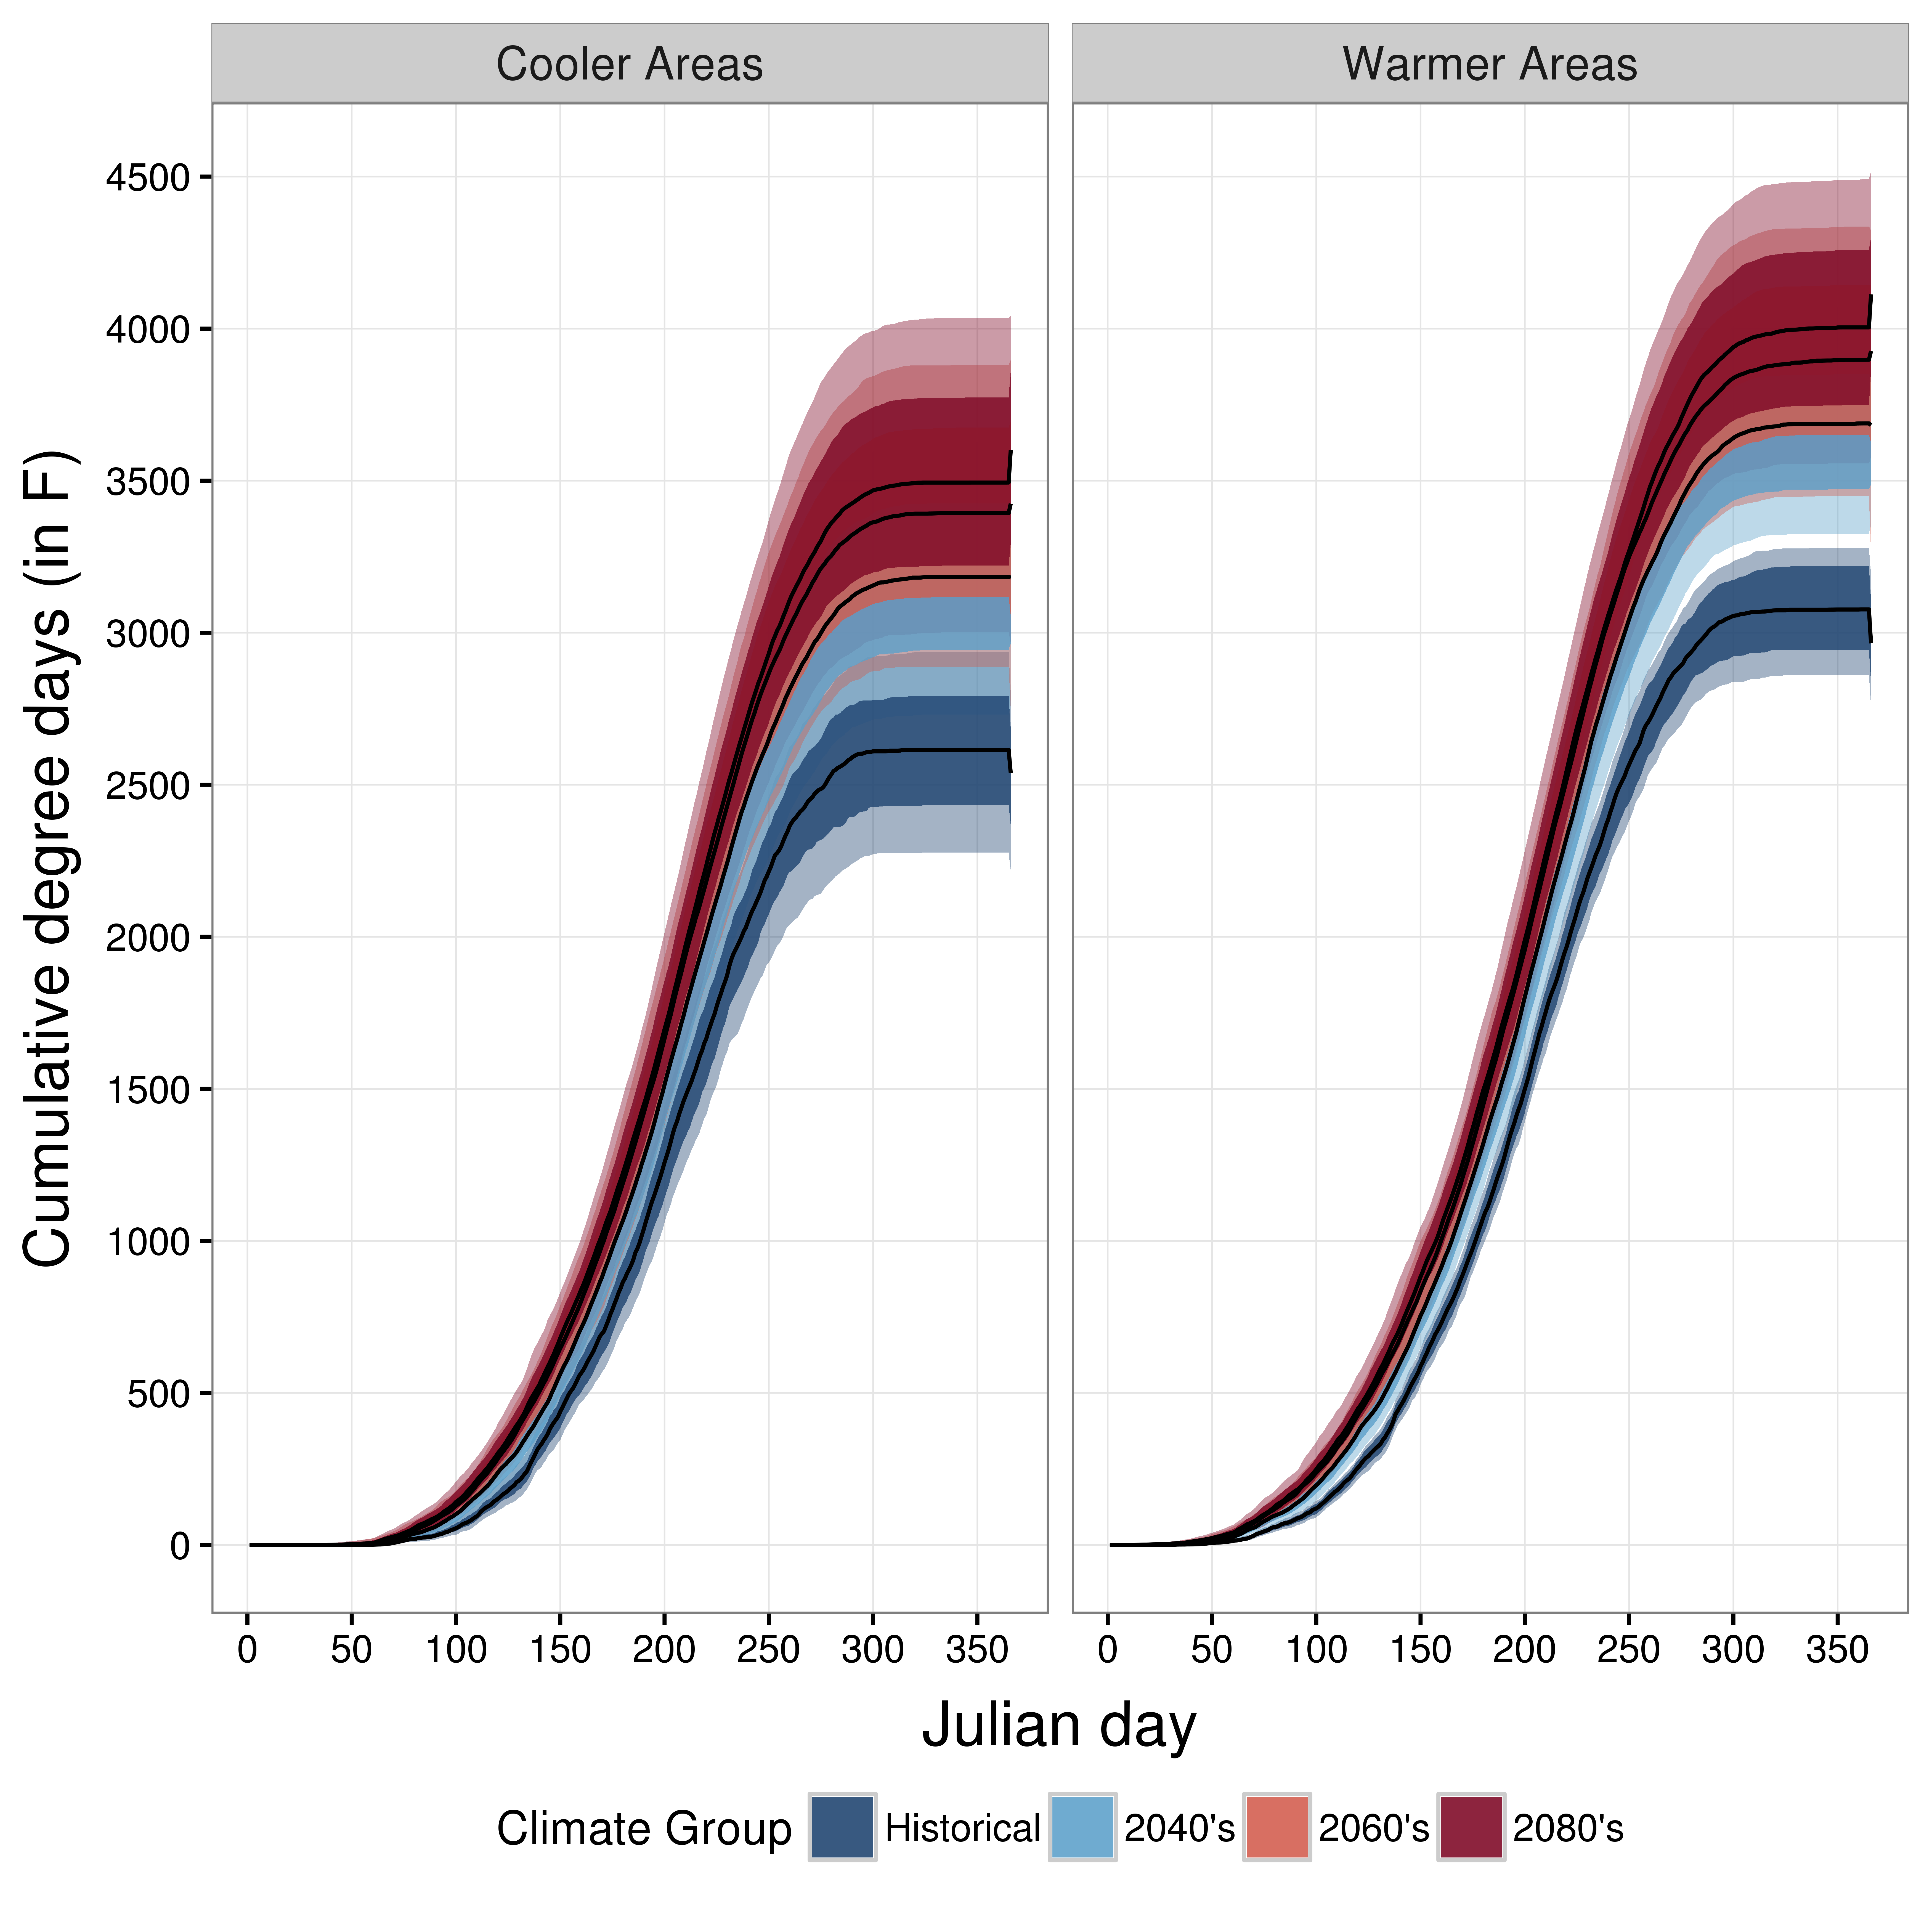
\includegraphics[width=1\linewidth]{figures/plot_cumdd_rcp45}
  \label{fig:DDC45}
\caption{Degree Day Changes (rcp 4.5)}
\end{subfigure}\hfill
\begin{subfigure}{.46\textwidth}
  \centering
  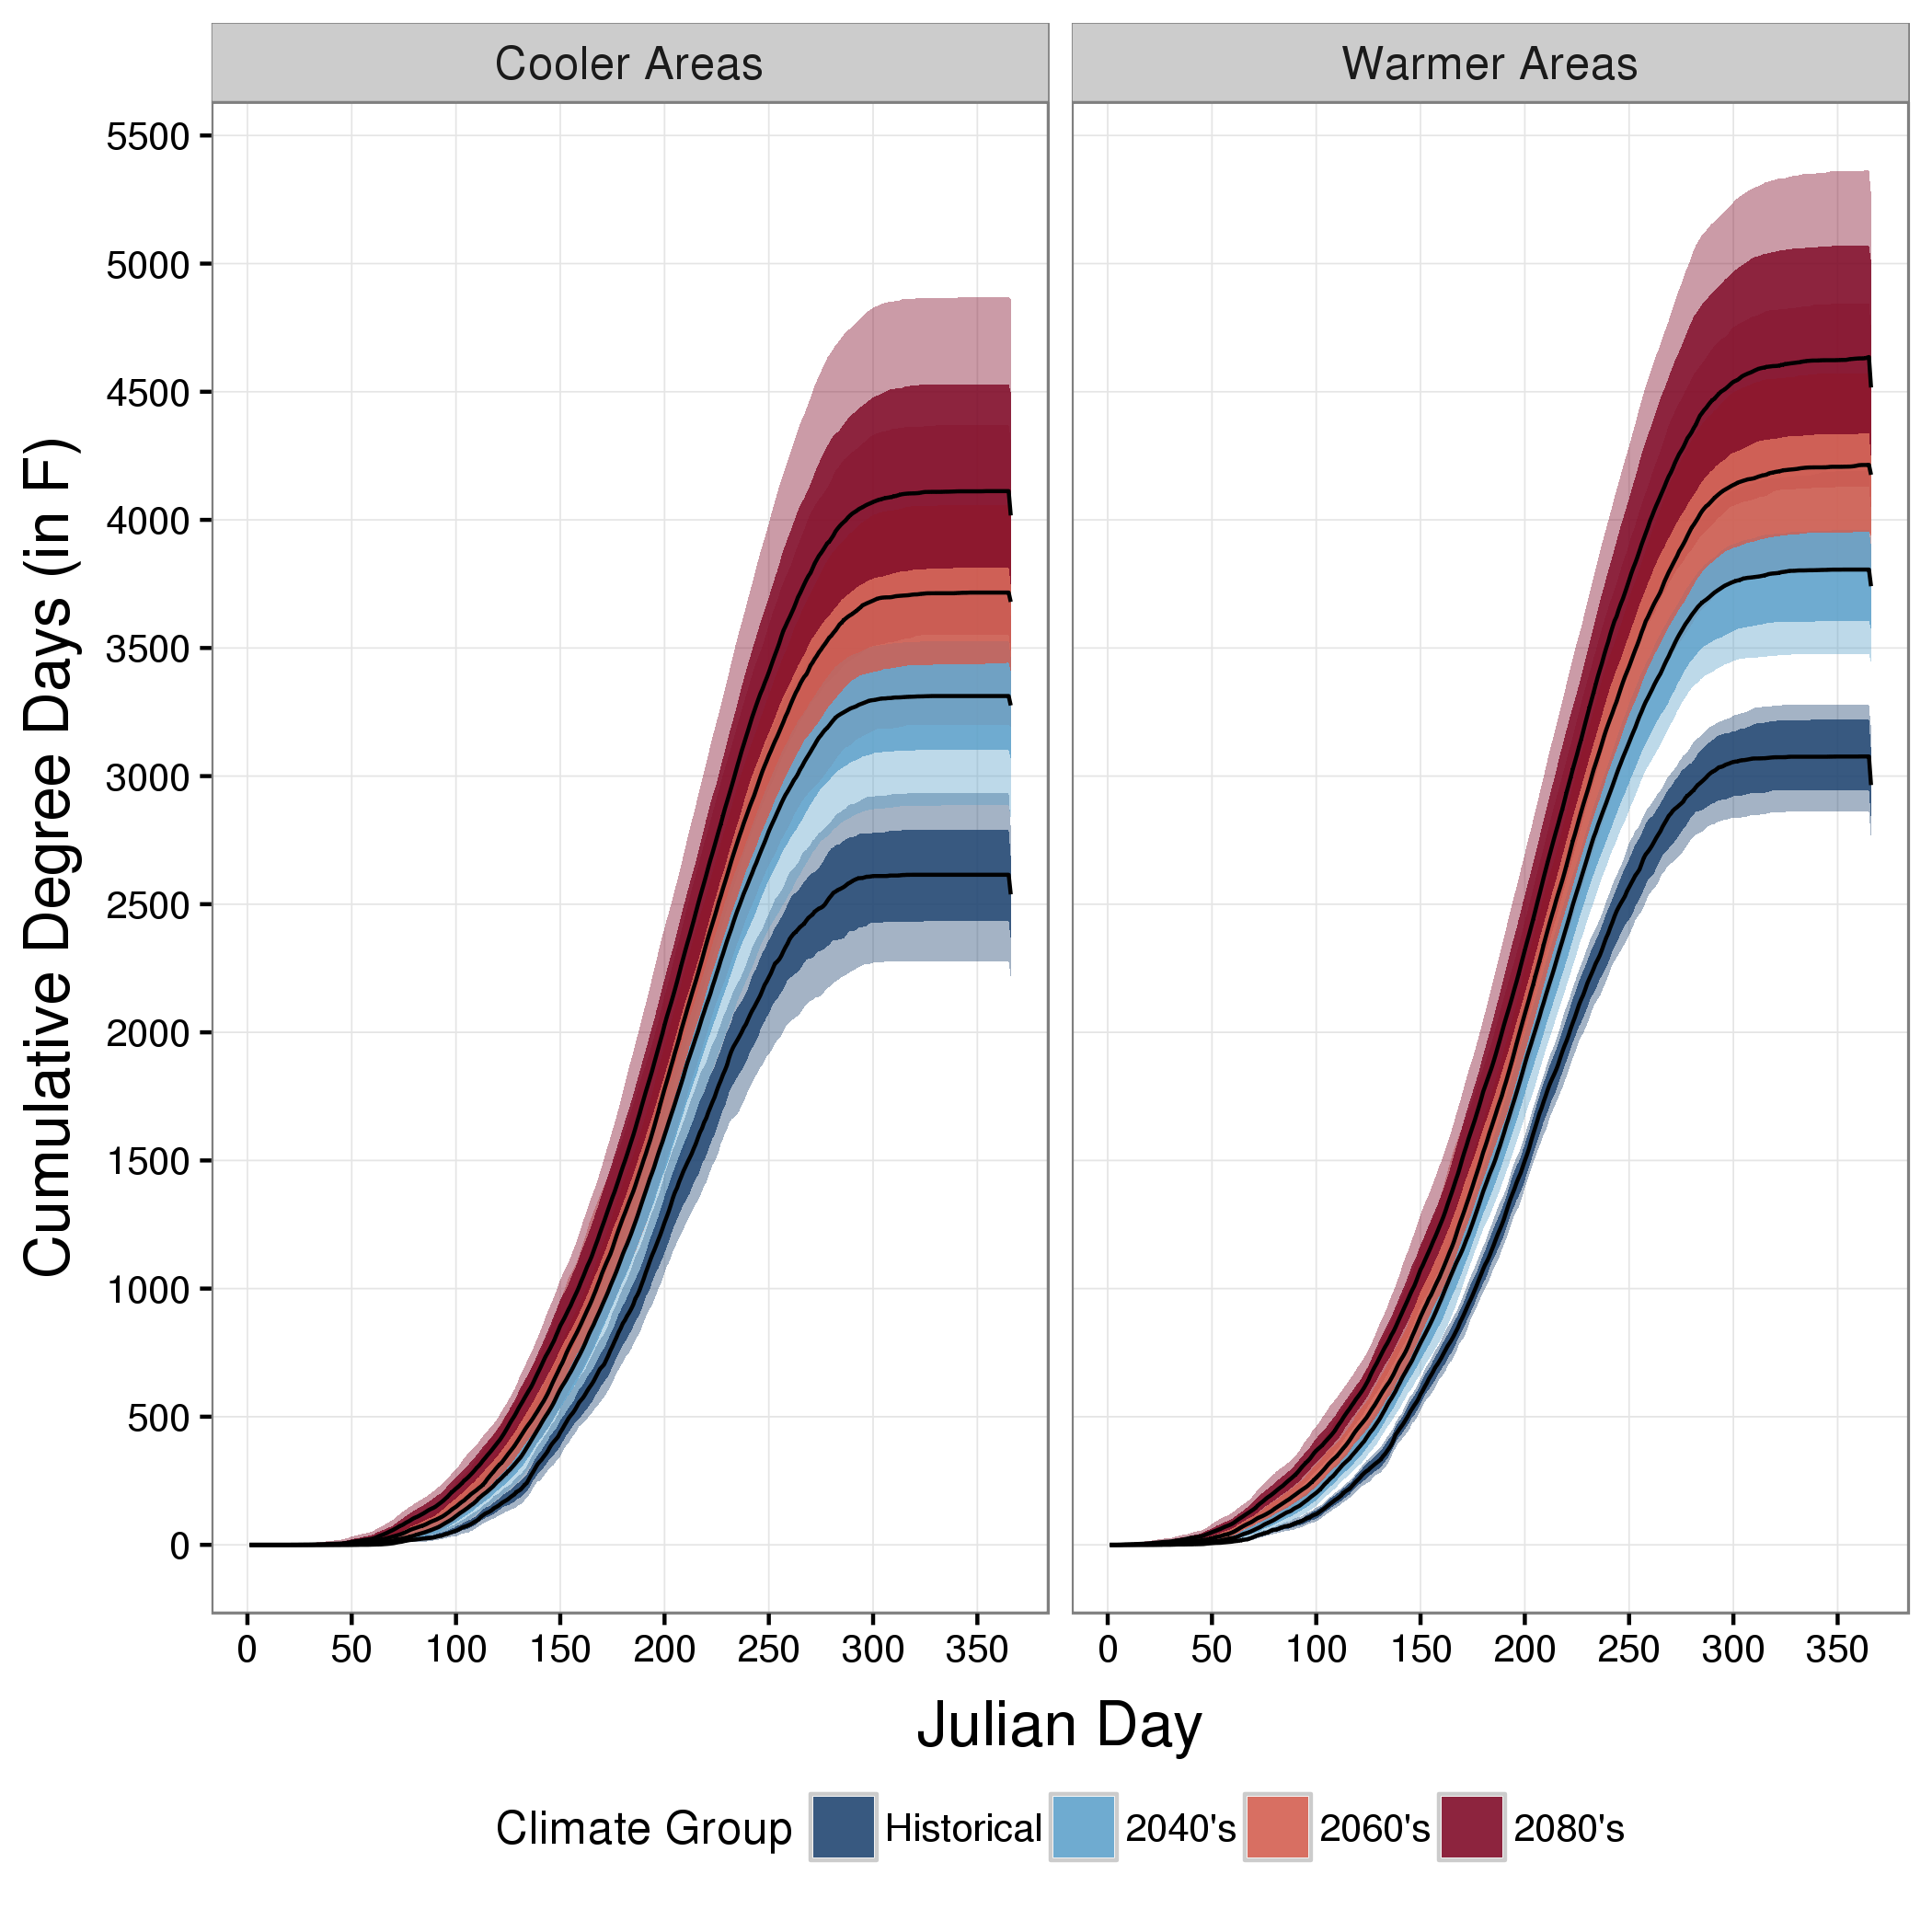
\includegraphics[width=1\linewidth]{figures/plot_cumdd_rcp85}
  \label{fig:DDC85}
\caption{Degree Day Changes (rcp 8.5)}
\end{subfigure}
%%%%%%%
\caption{Degree Day changes over a year}
\label{fig:DDC}
\end{figure}
\pagebreak
%%%%%%%%%%%%%%%%%%%%%%%%%%%%%%%%%%%%%%%%%%%%%%%%%
%%%%%%%%%%%%%%%%%%%%%%%%%%%%%%%%%%%%%%%%%%%%%%%%%
\subsection{Changes in timing of events critical for pest management}
Adult first flight and egg hatch into larvae (Are these the critical times at which pesticide applications are made?) 

\begin{figure}[h!]
    \centering
    \begin{subfigure}[b]{0.48\textwidth}
        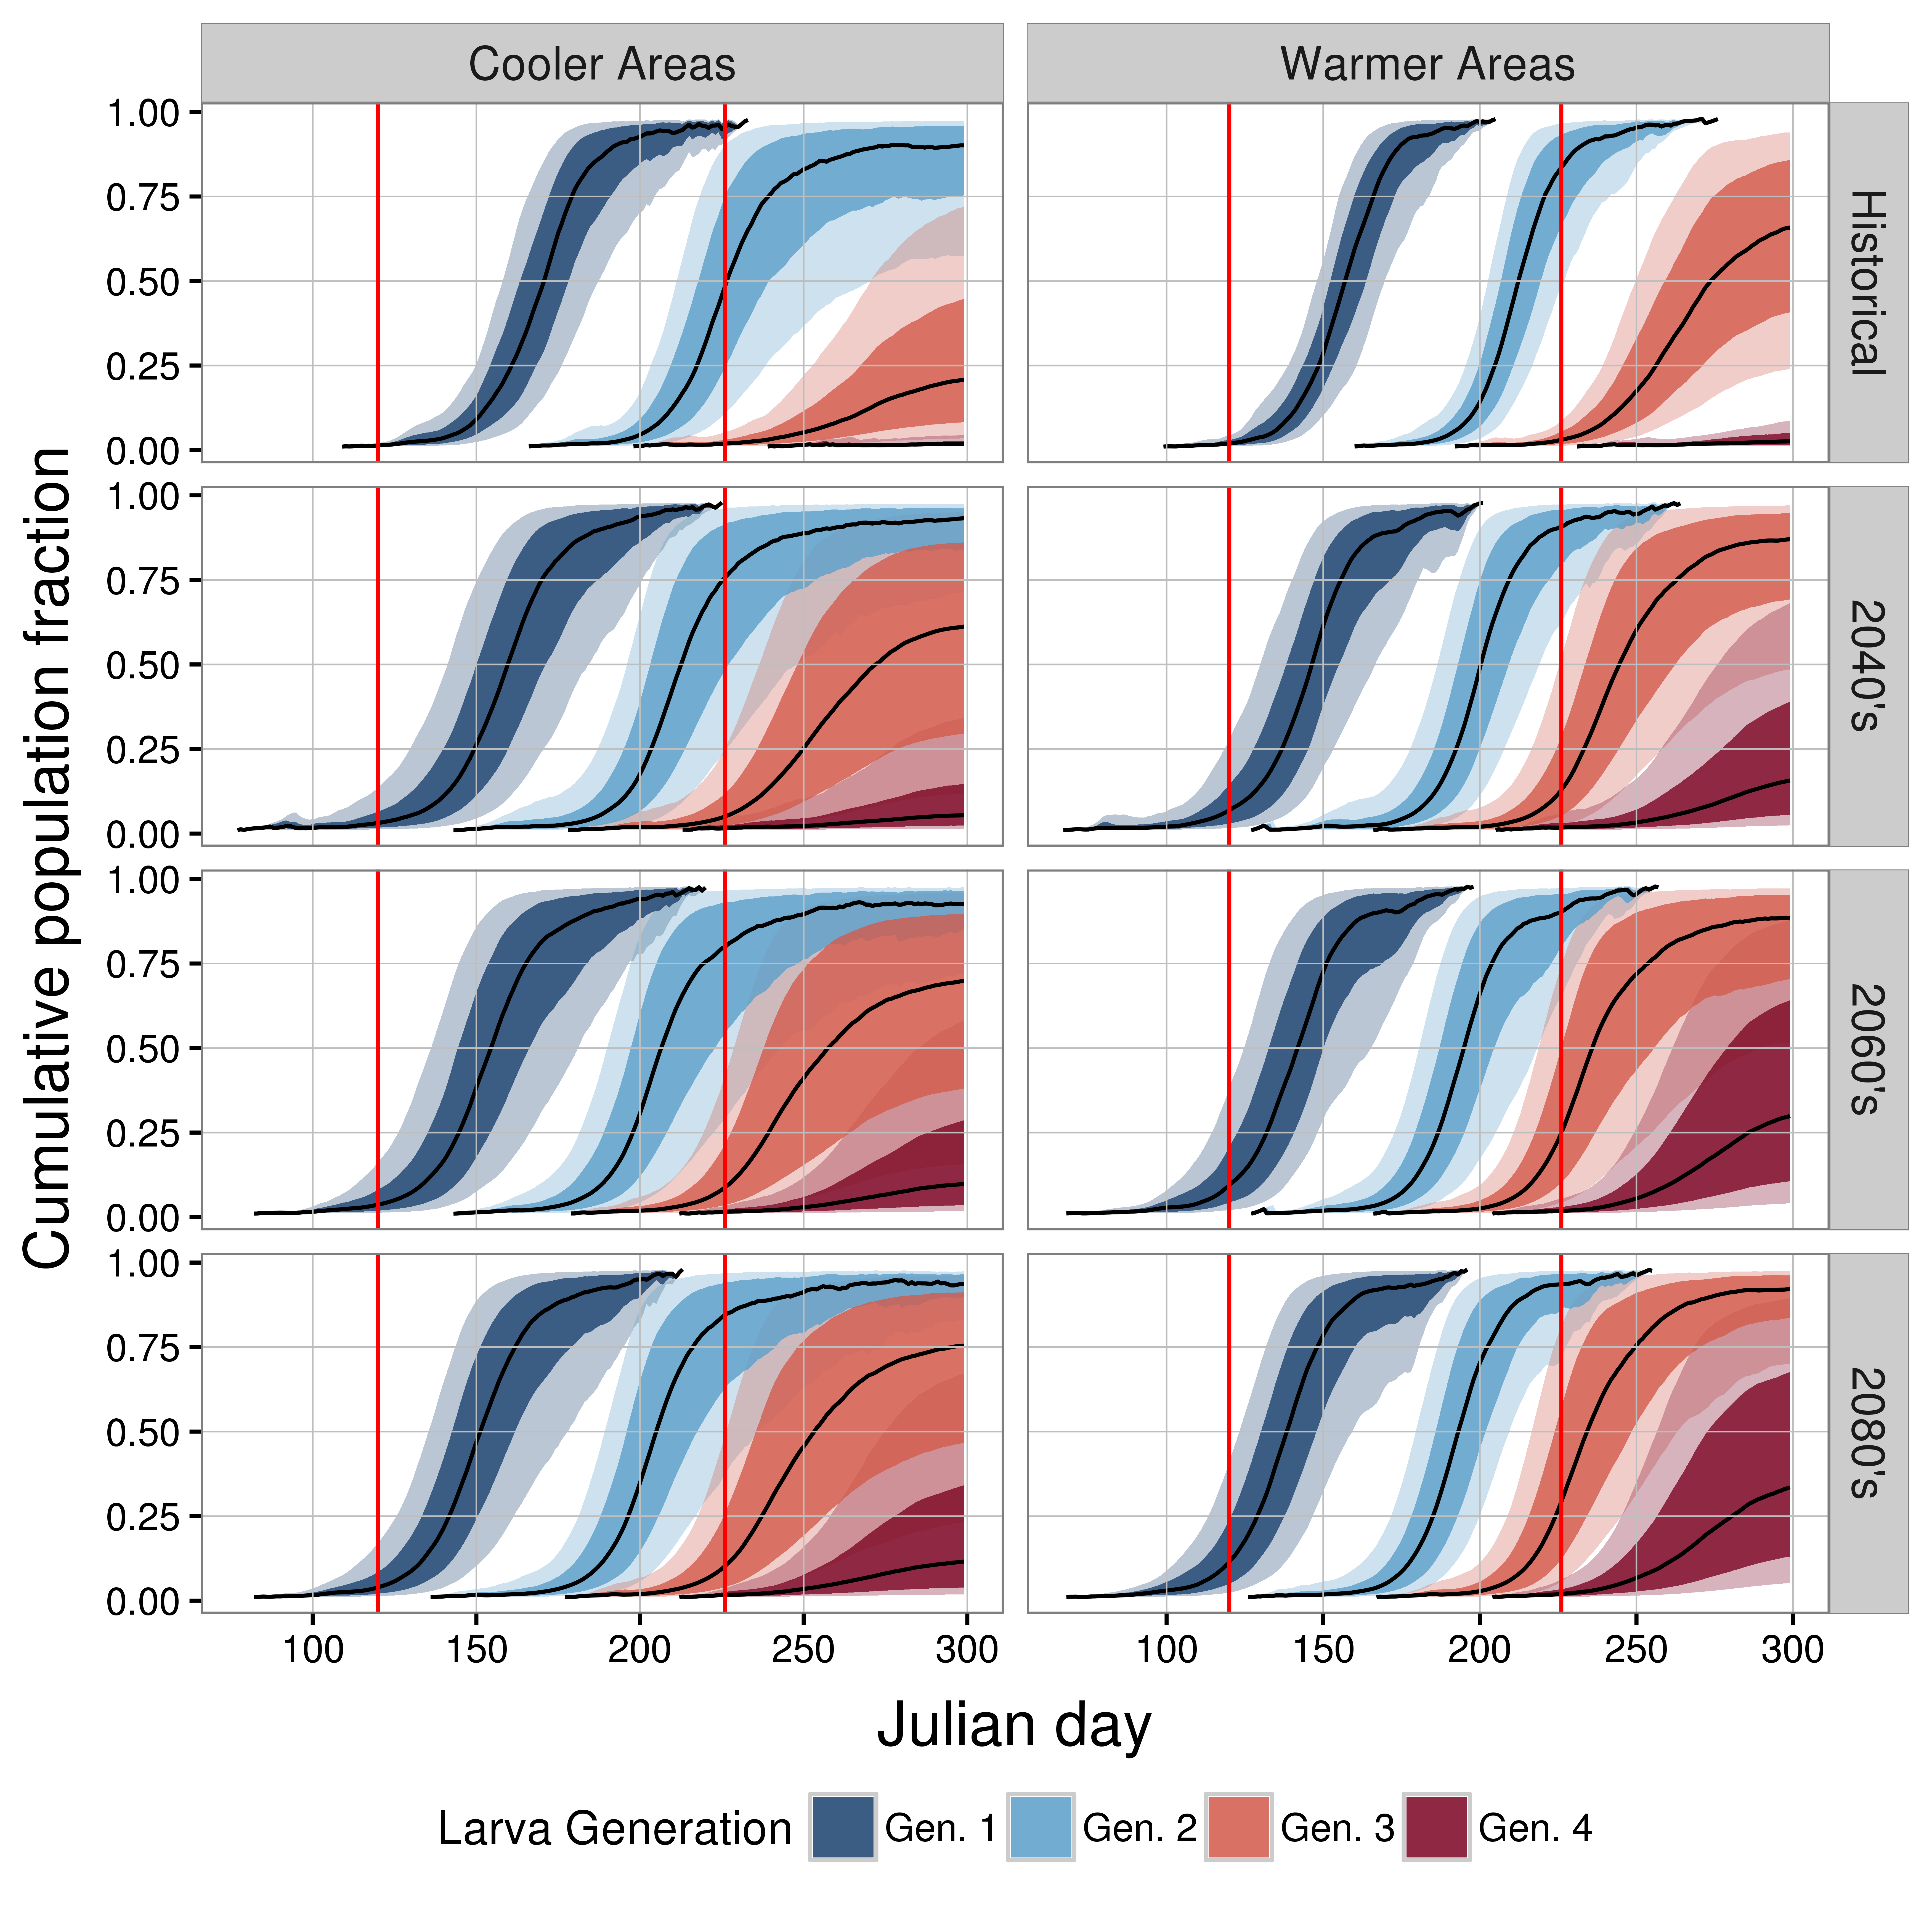
\includegraphics[width=\textwidth]{figures/plot_eggHatch_rcp45}
        \caption{Eggs hatching (rcp 4.5)}
        \label{fig:Eggs_Hatch_45)}
    \end{subfigure}
    ~ %add desired spacing between images, e. g. ~, \quad, \qquad, \hfill etc. 
      %(or a blank line to force the subfigure onto a new line)
    \begin{subfigure}[b]{0.48\textwidth}
        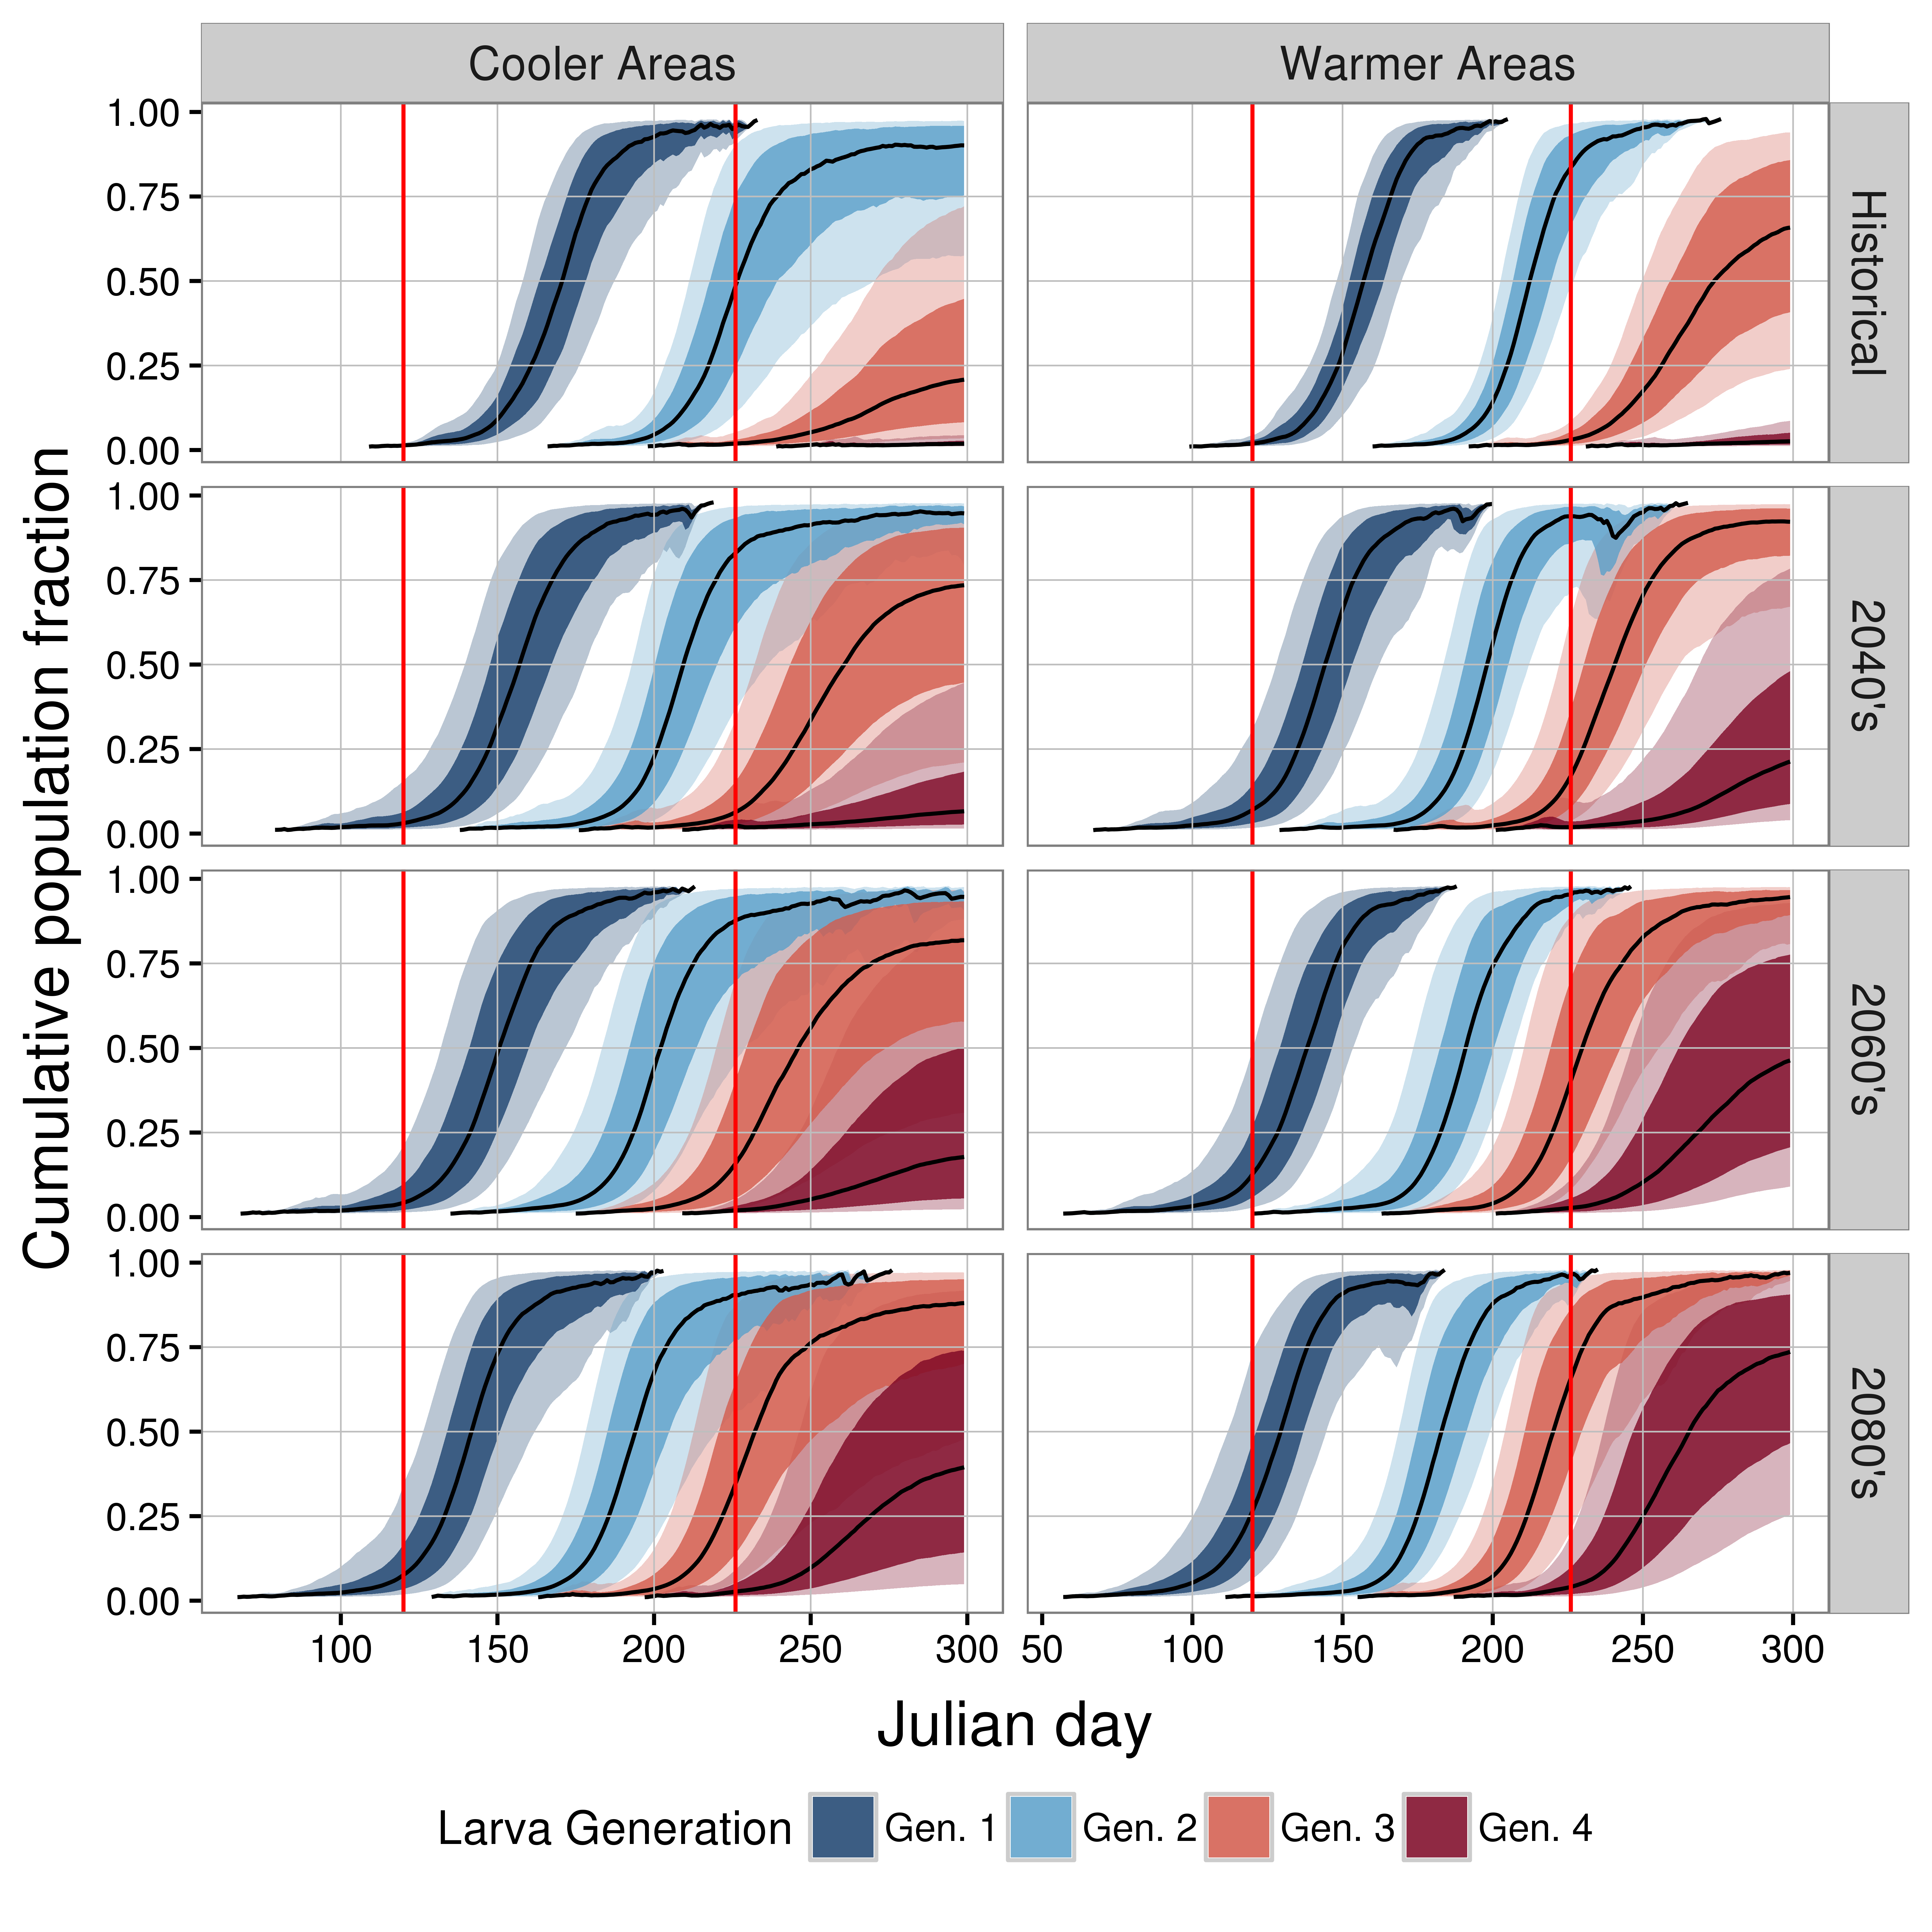
\includegraphics[width=\textwidth]{figures/plot_eggHatch_rcp85}
        \caption{Eggs hatching (rcp 8.5)}
        \label{fig:Eggs_Hatch_85}
    \end{subfigure}\\
   \caption{Egg hatches}\label{fig:Egg_hatchs}
\end{figure}

\begin{figure}[h!]
    \hspace{.1in}
    \begin{subfigure}[b]{0.5\textwidth}
        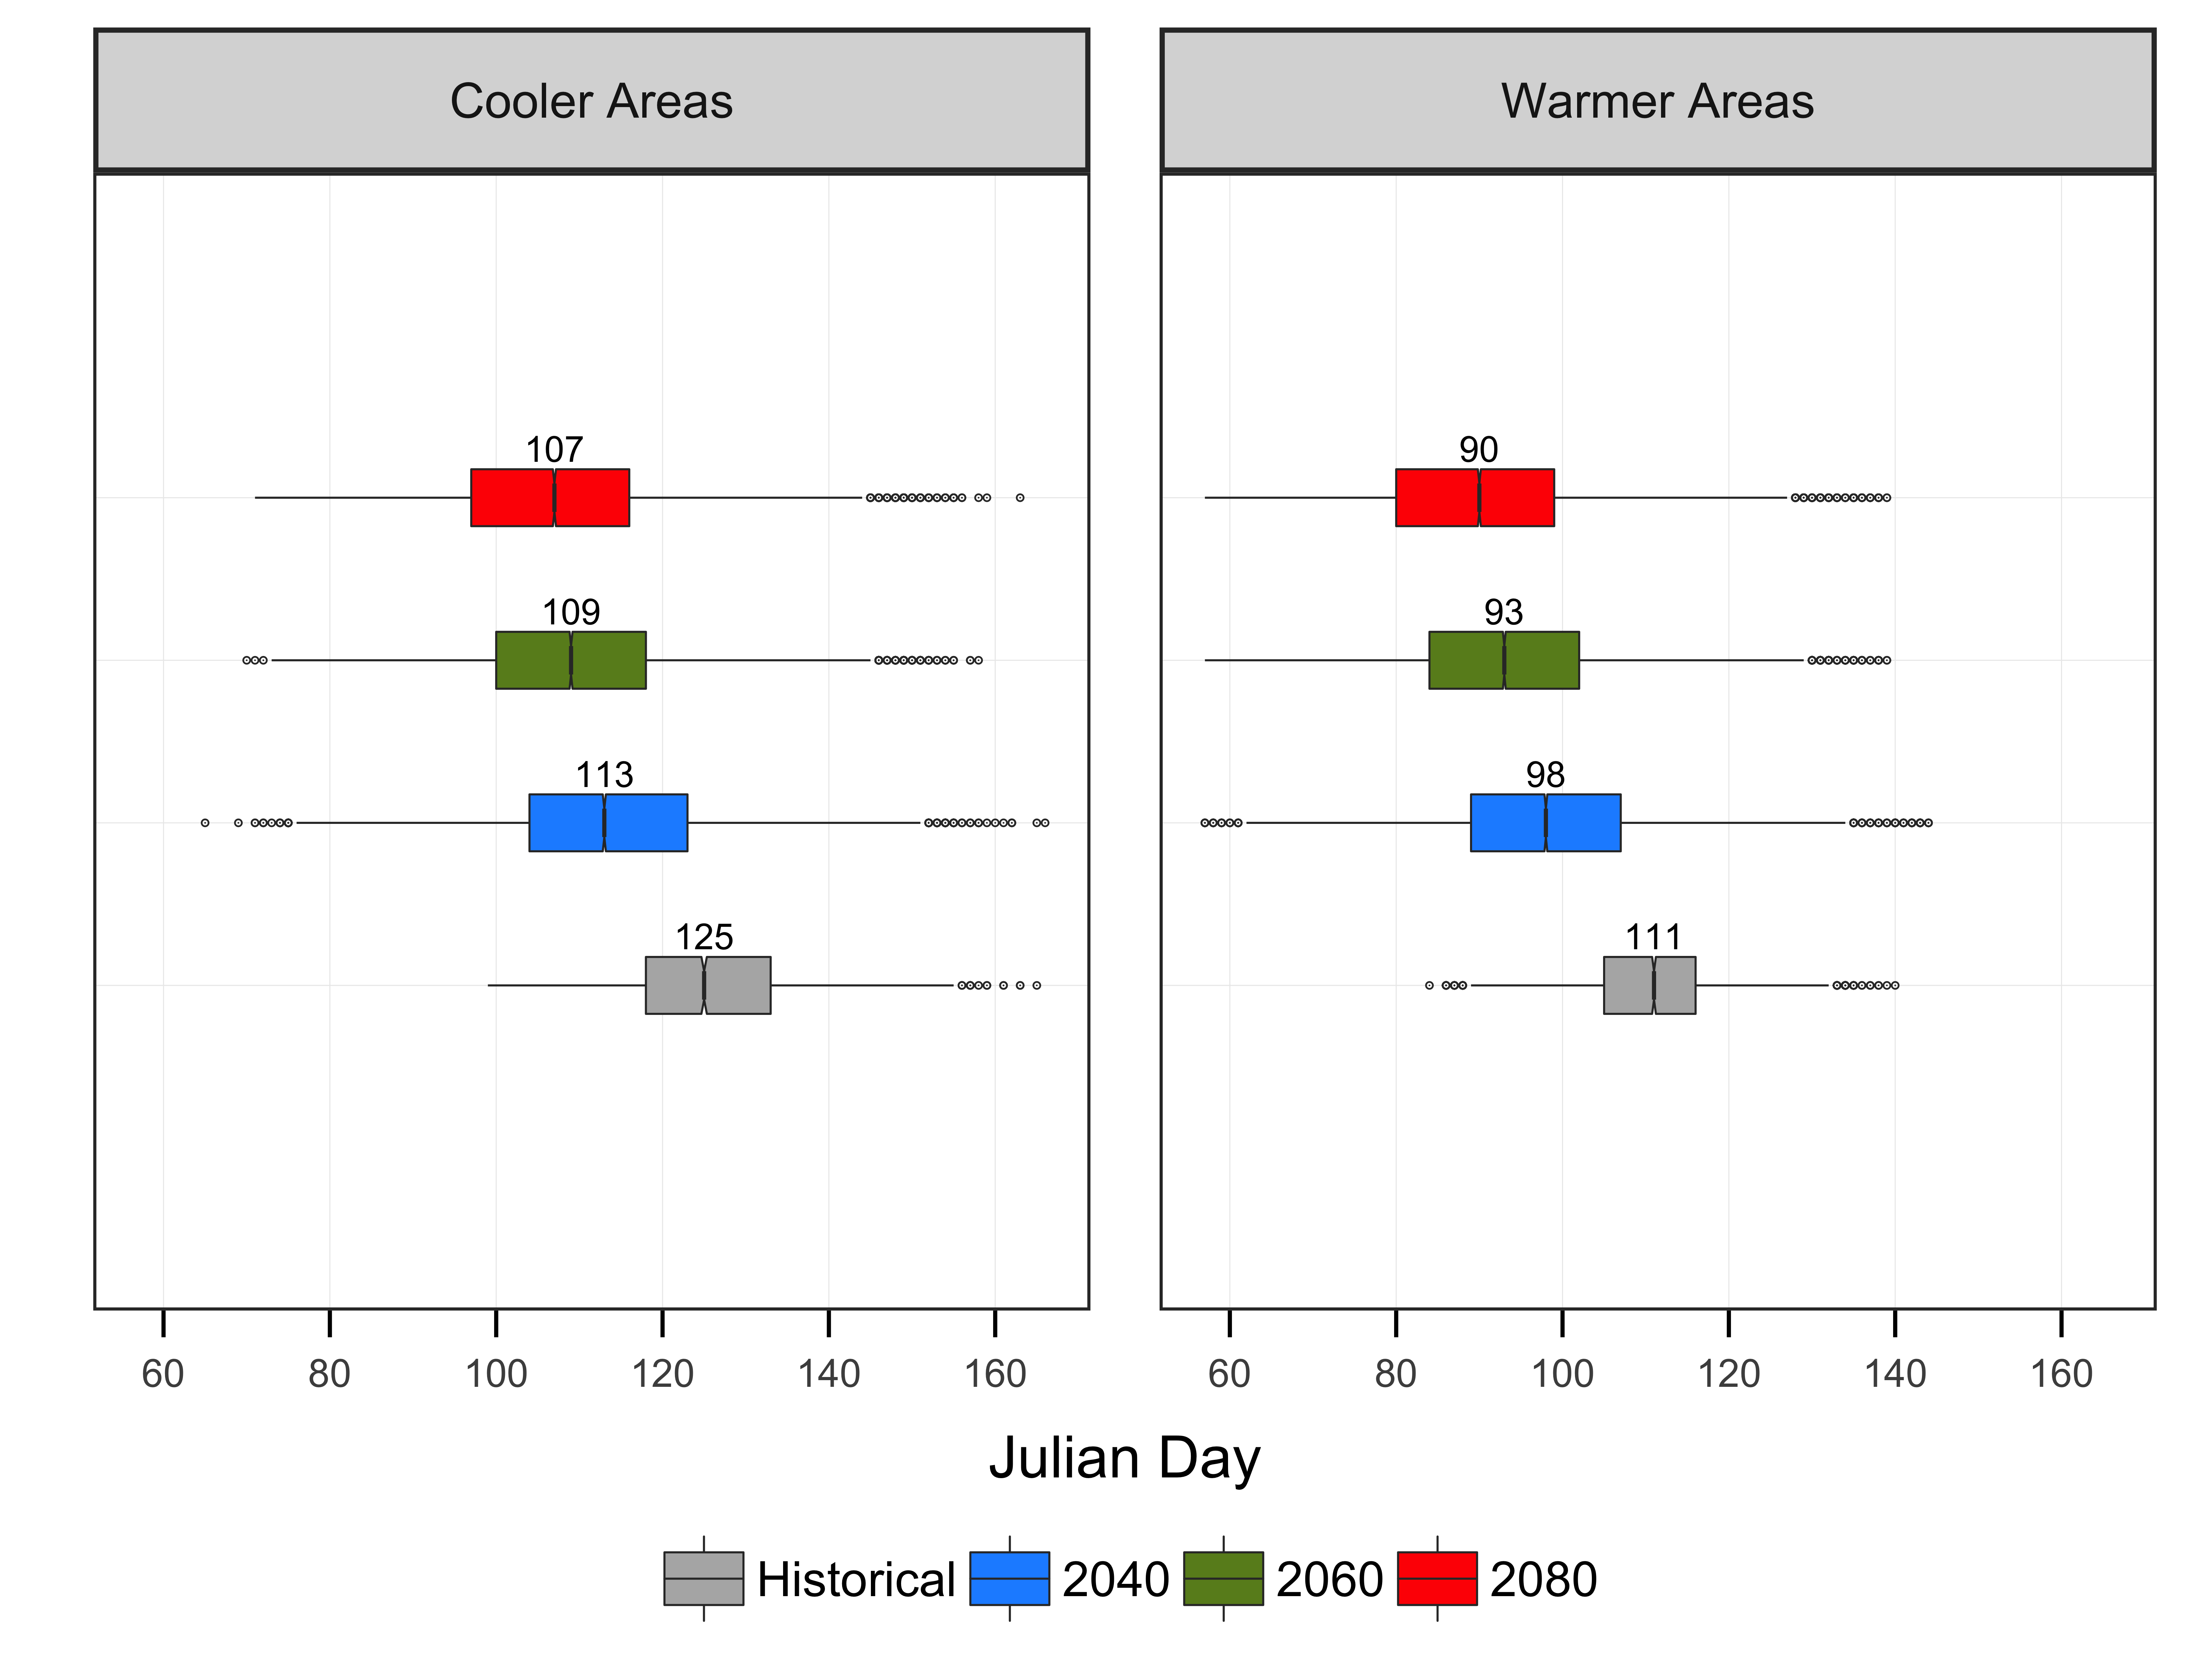
\includegraphics[width=\textwidth]{figures/adult_emergence_rcp45}
        \caption{Adult first flight (rcp 4.5)}
        \label{fig:aff_45}
    \end{subfigure}
     \hspace{-.2in}
    ~ %add desired spacing between images, e. g. ~, \quad, \qquad, \hfill etc. 
    %(or a blank line to force the subfigure onto a new line)
    \begin{subfigure}[b]{0.5\textwidth}
        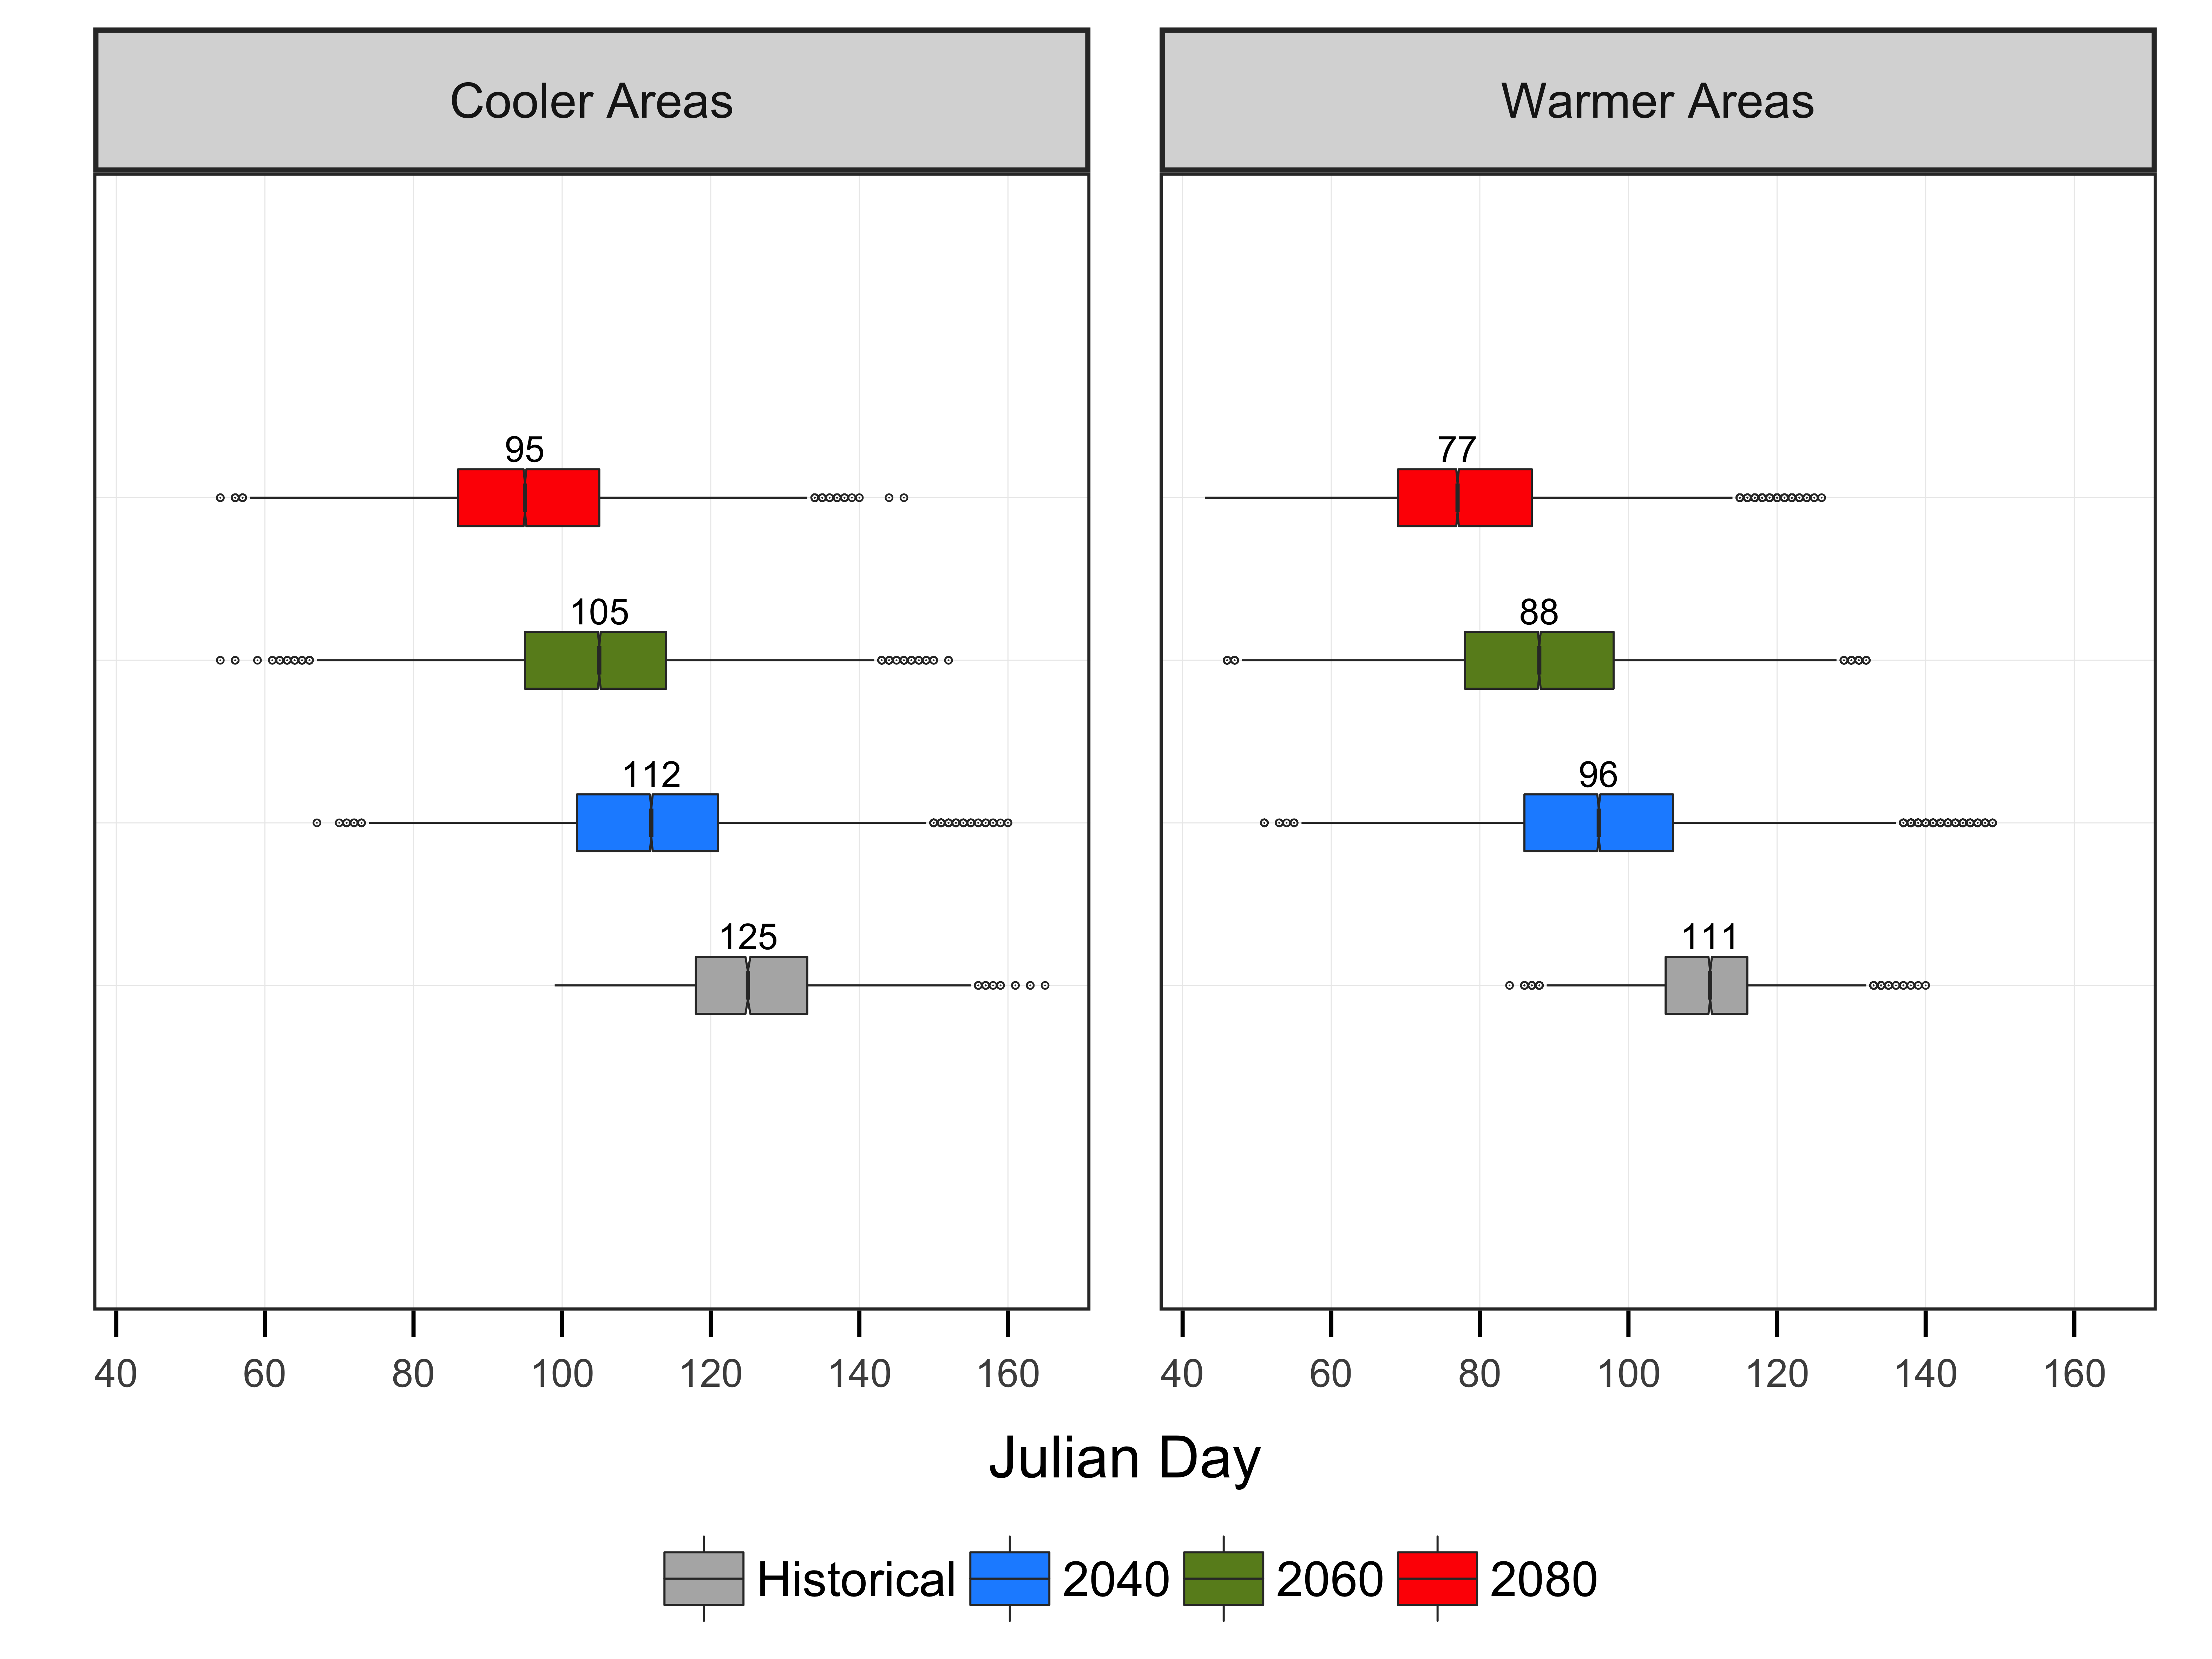
\includegraphics[width=\textwidth]{figures/adult_emergence_rcp85}
        \caption{Adult first flight (rcp 8.5)}
        \label{fig:aff_85}
    \end{subfigure}
    \caption{First adult flights}\label{fig:First_adult_flights}
\end{figure}


\begin{figure}[h!]
    \hspace{.1in}
    \begin{subfigure}[b]{0.5\textwidth}
        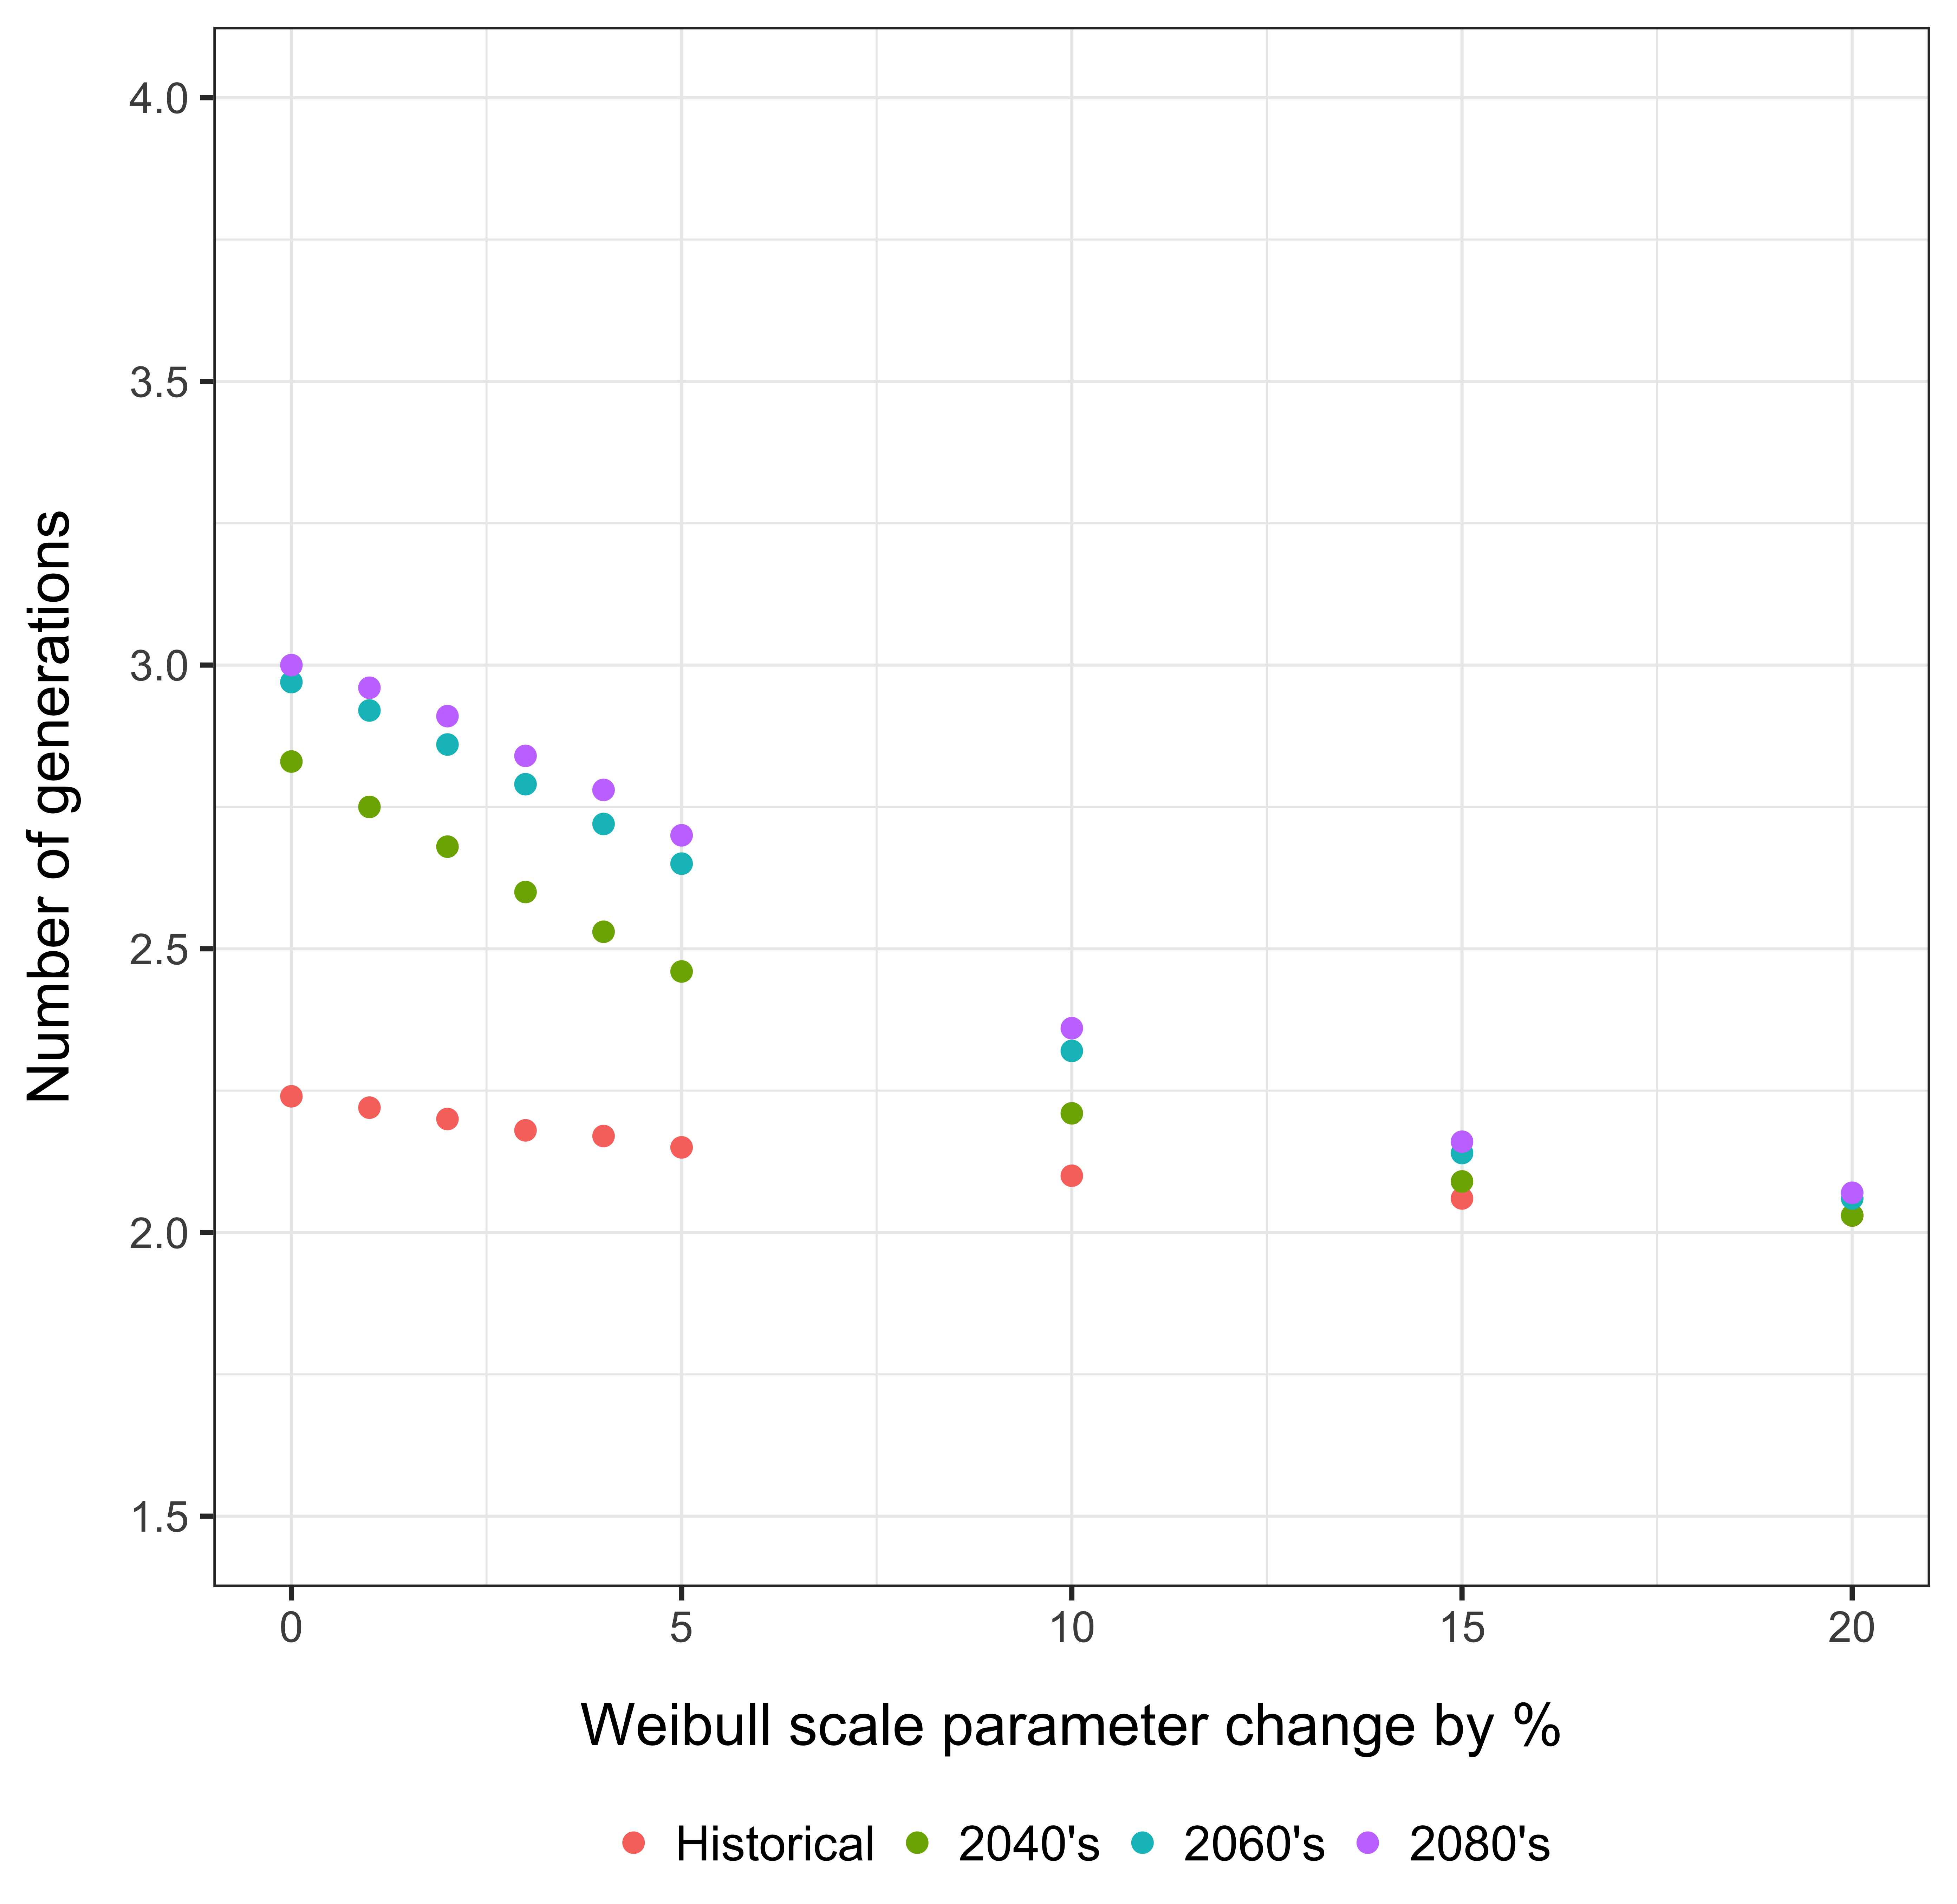
\includegraphics[width=\textwidth]{figures/rcp45_Adult_Aug_scale_sens}
        \caption{Adult first flight (rcp 4.5)}
        \label{fig:aff_45}
    \end{subfigure}
     \hspace{-.1in}
    ~ %add desired spacing between images, e. g. ~, \quad, \qquad, \hfill etc. 
    %(or a blank line to force the subfigure onto a new line)
    \begin{subfigure}[b]{0.5\textwidth}
        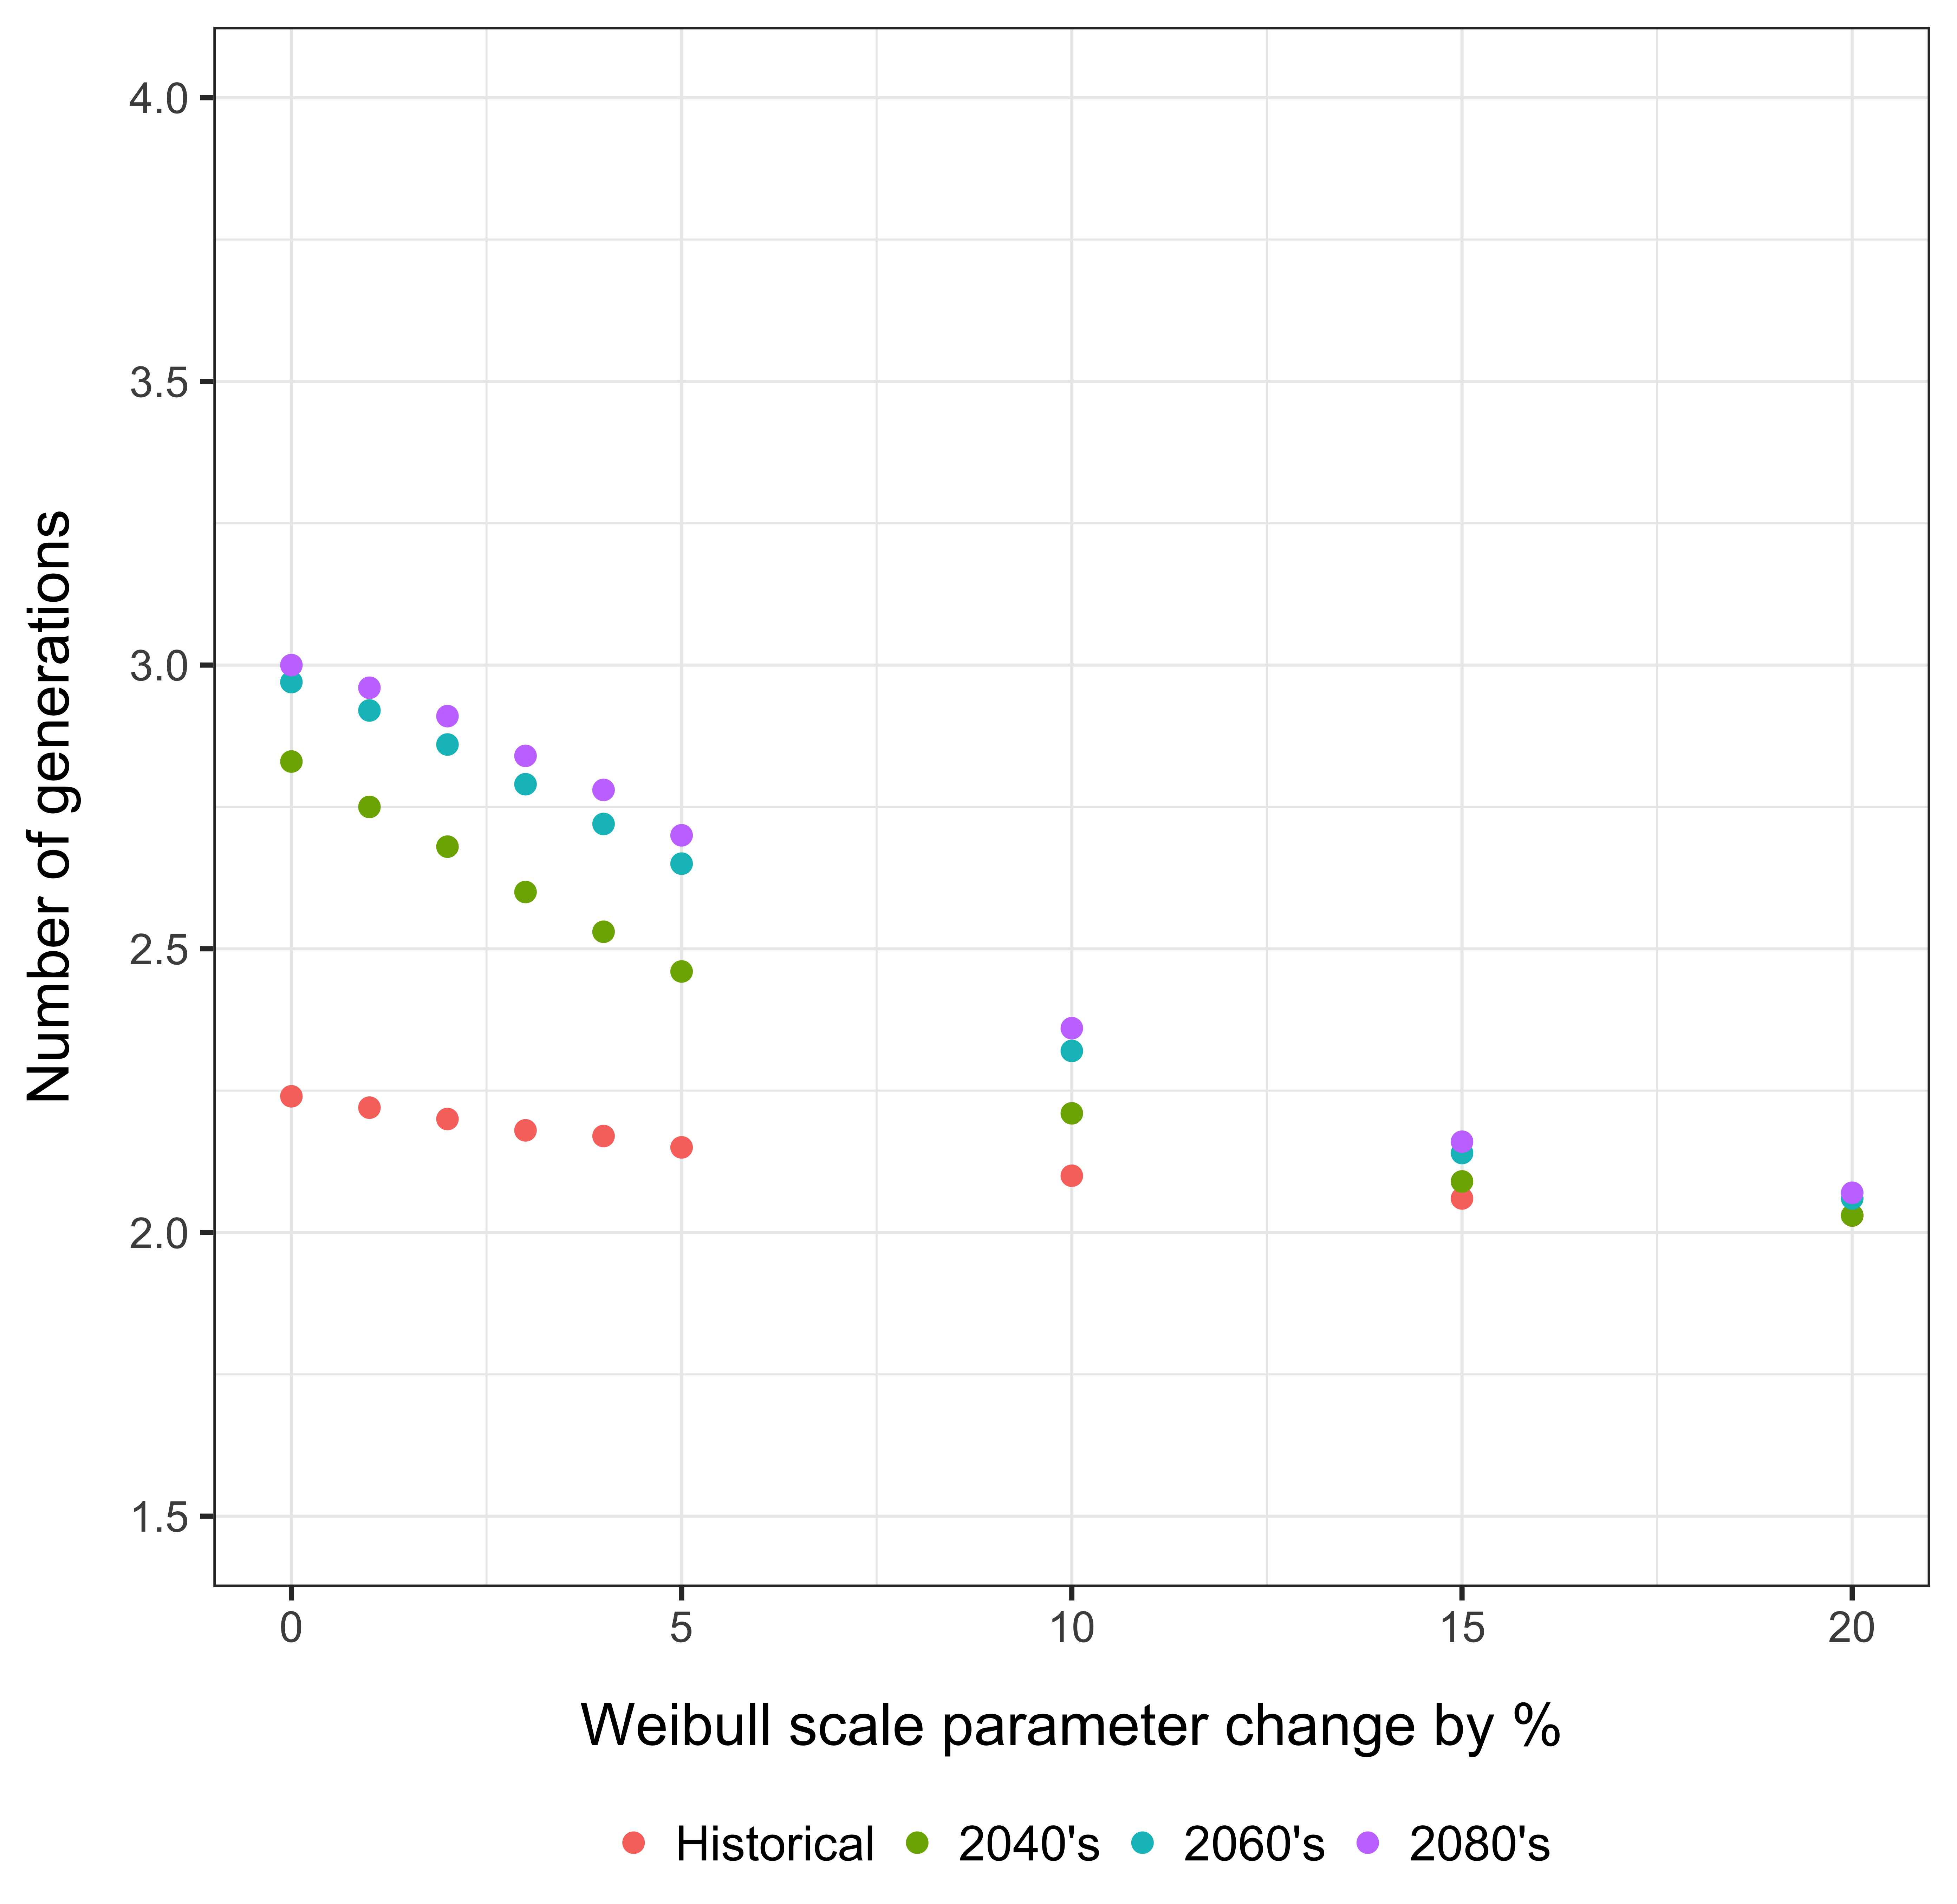
\includegraphics[width=\textwidth]{figures/rcp45_Adult_Aug_scale_sens}
        \caption{Adult first flight (rcp 8.5)}
        \label{fig:aff_85}
    \end{subfigure}
    \caption{First adult flights}\label{fig:First_adult_flights}
\end{figure}



\pagebreak
%%%%%%%%%%%%%%%%%%%%%%%%%%%%%%%%%%%%%%%%%%%%%%%%%
%%%%%%%%%%%%%%%%%%%%%%%%%%%%%%%%%%%%%%%%%%%%%%%%%

\subsection{Changes in the number of generations of the pest}
Show this for the larval stage. Show for August 23 and Nov 5.

\begin{figure}[h!]
    \centering
    \begin{subfigure}[b]{0.45\textwidth}
        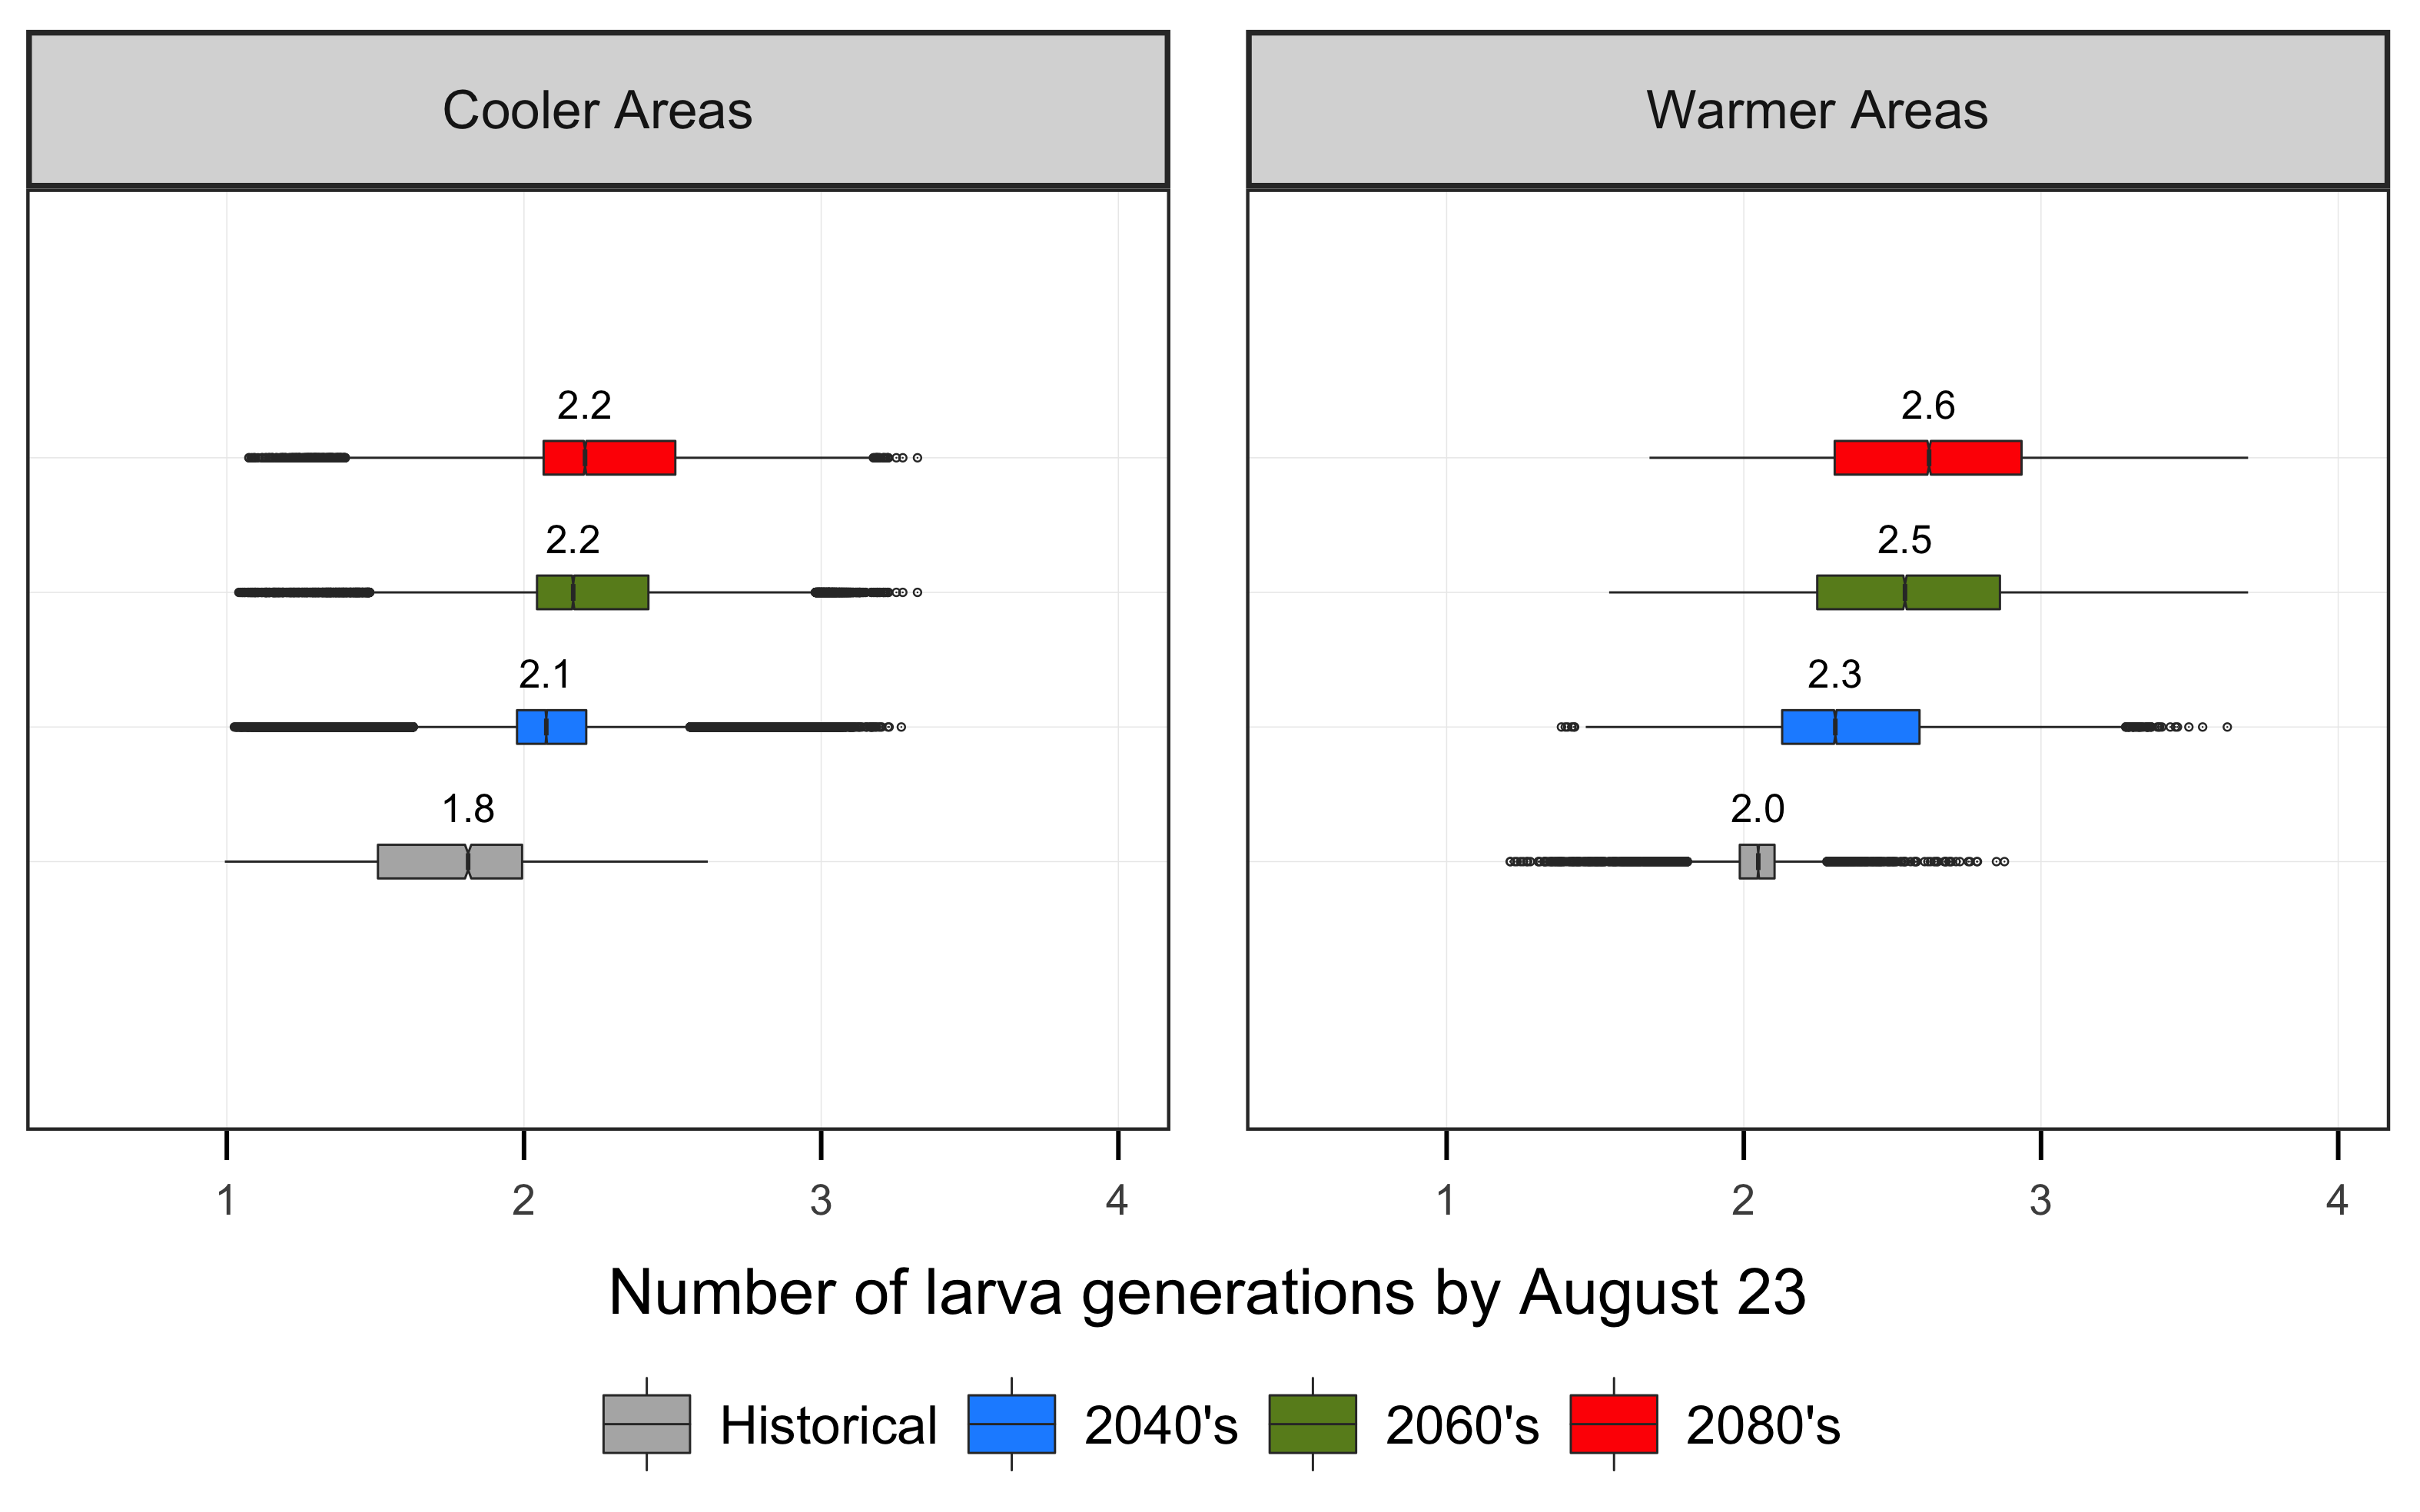
\includegraphics[width=\textwidth]{figures/Larva_Gen_Aug_rcp45}
    \end{subfigure}
     %add desired spacing between images, e. g. ~, \quad, \qquad, \hfill etc. 
      %(or a blank line to force the subfigure onto a new line)
    \begin{subfigure}[b]{0.45\textwidth}
        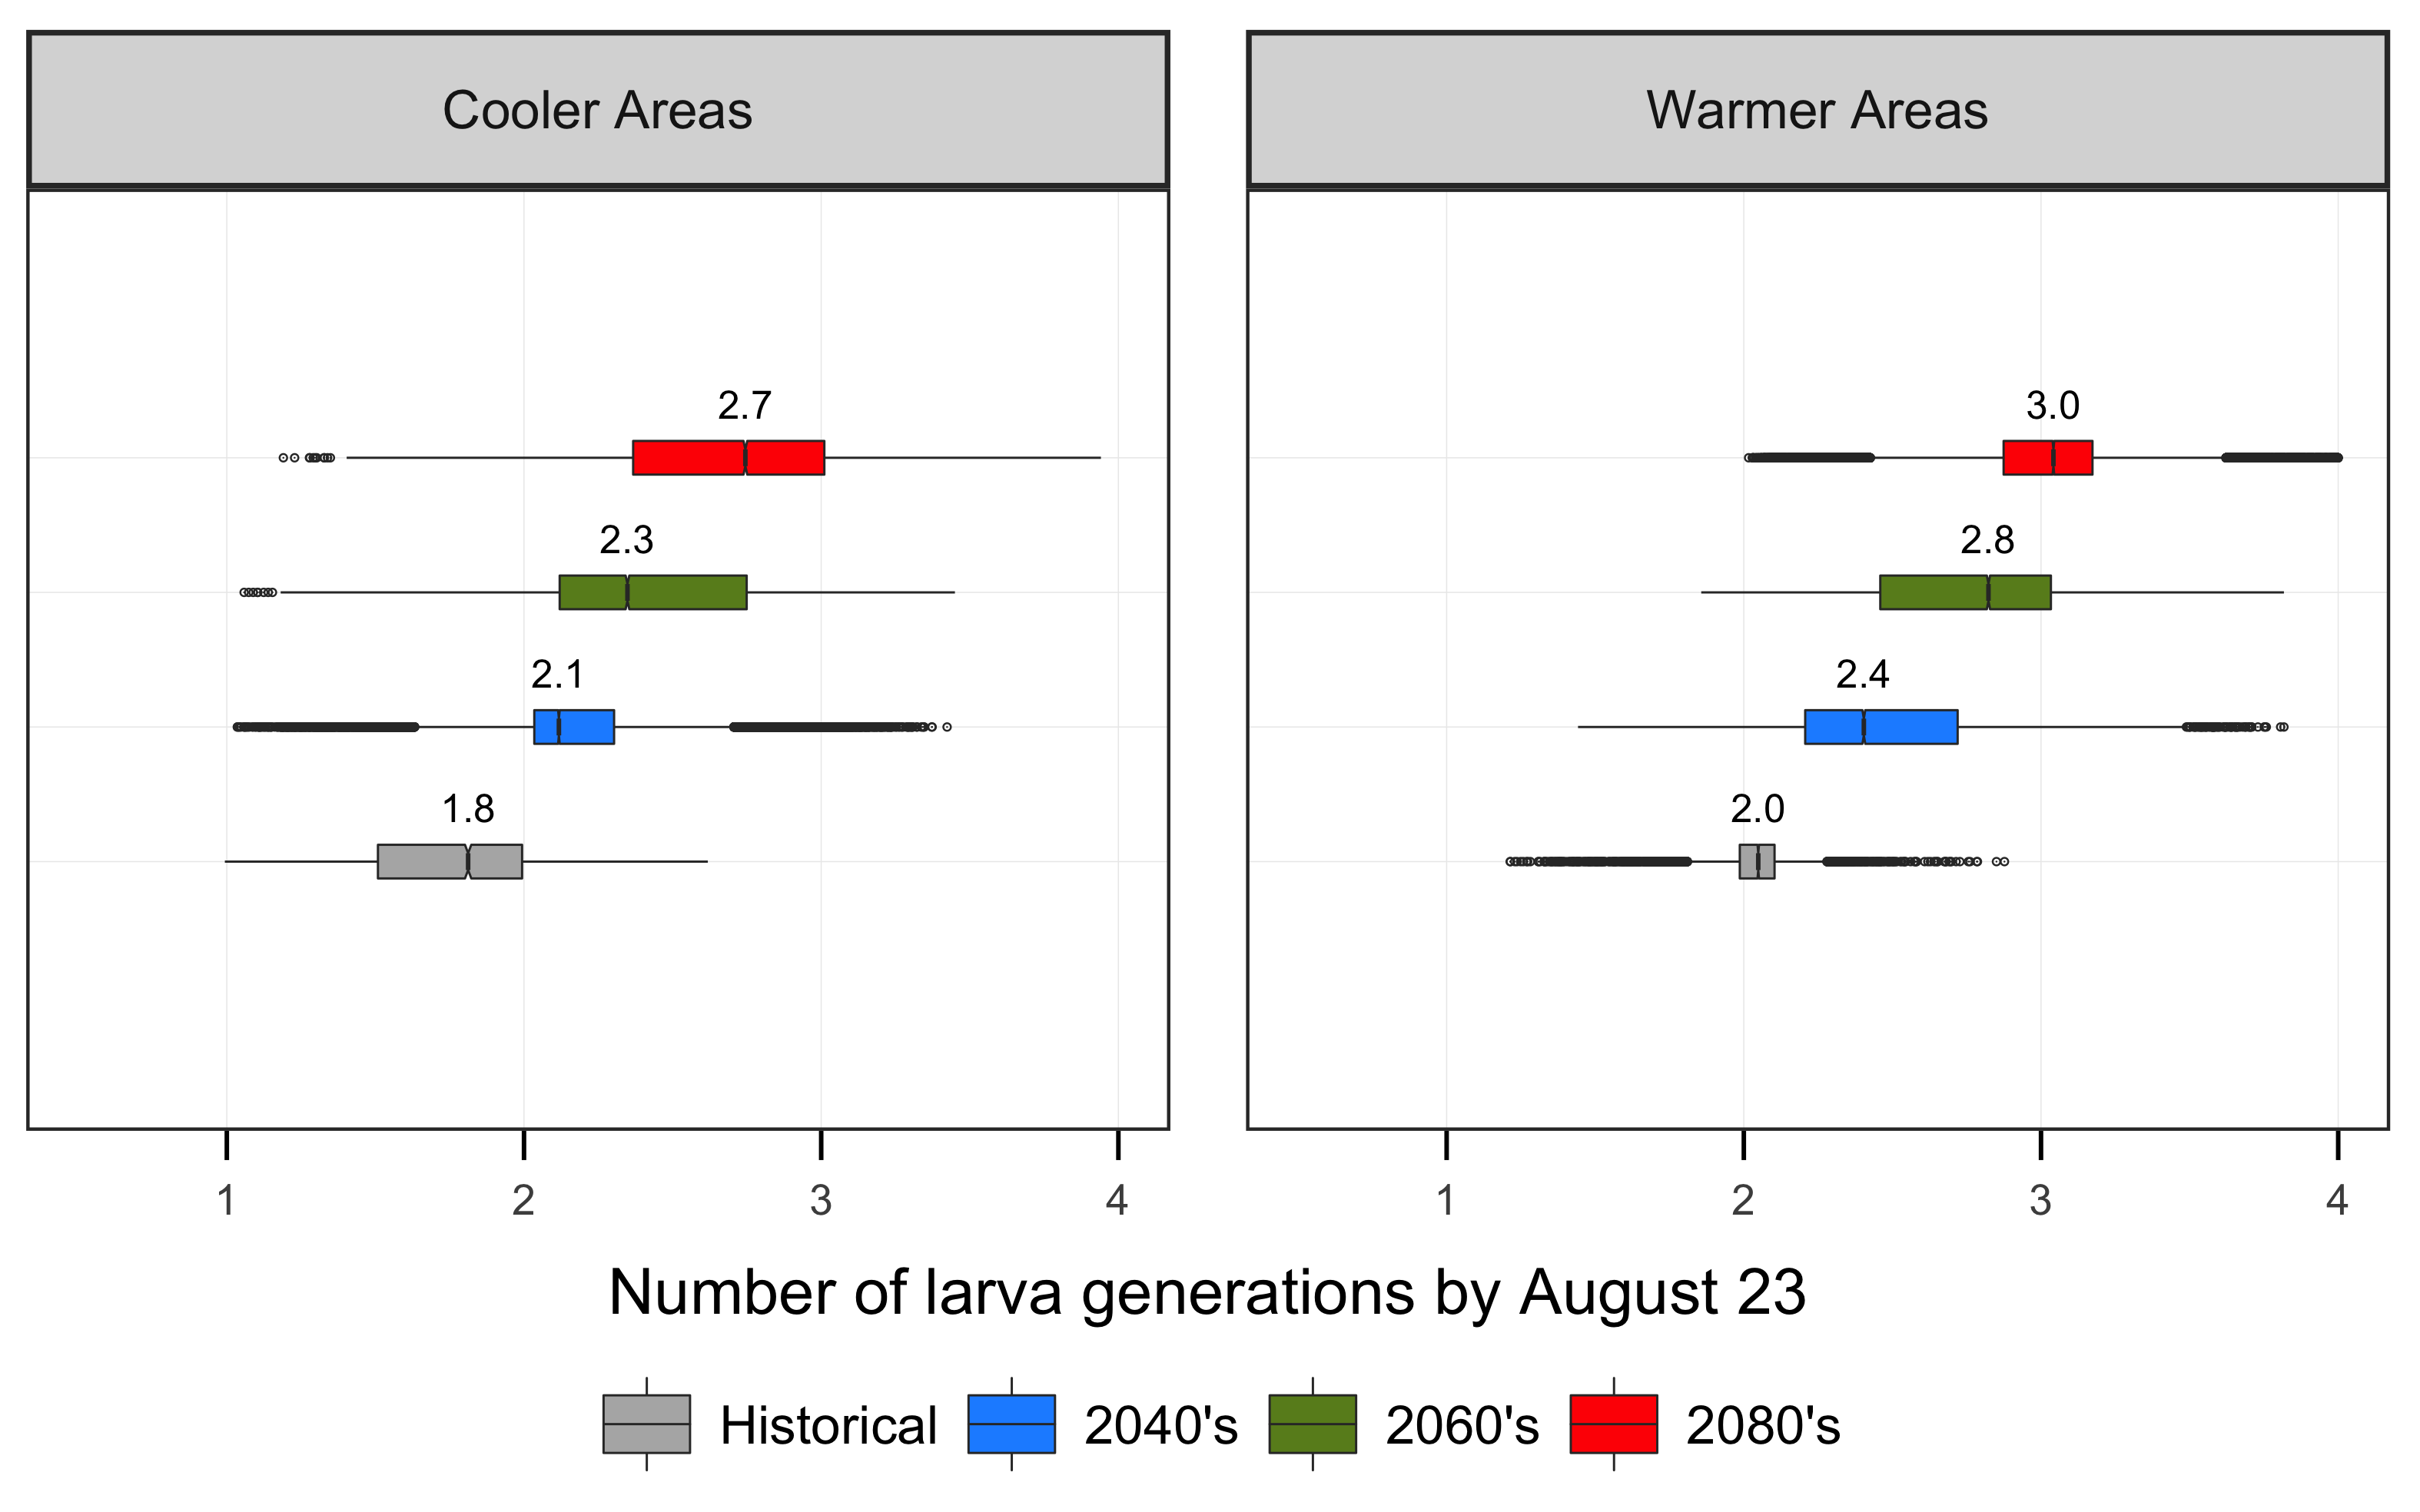
\includegraphics[width=\textwidth]{figures/Larva_Gen_Aug_rcp85}
    \end{subfigure}\\    
     %add desired spacing between images, e. g. ~, \quad, \qquad, \hfill etc. 
      %(or a blank line to force the subfigure onto a new line)
          \begin{subfigure}[b]{0.45\textwidth}
        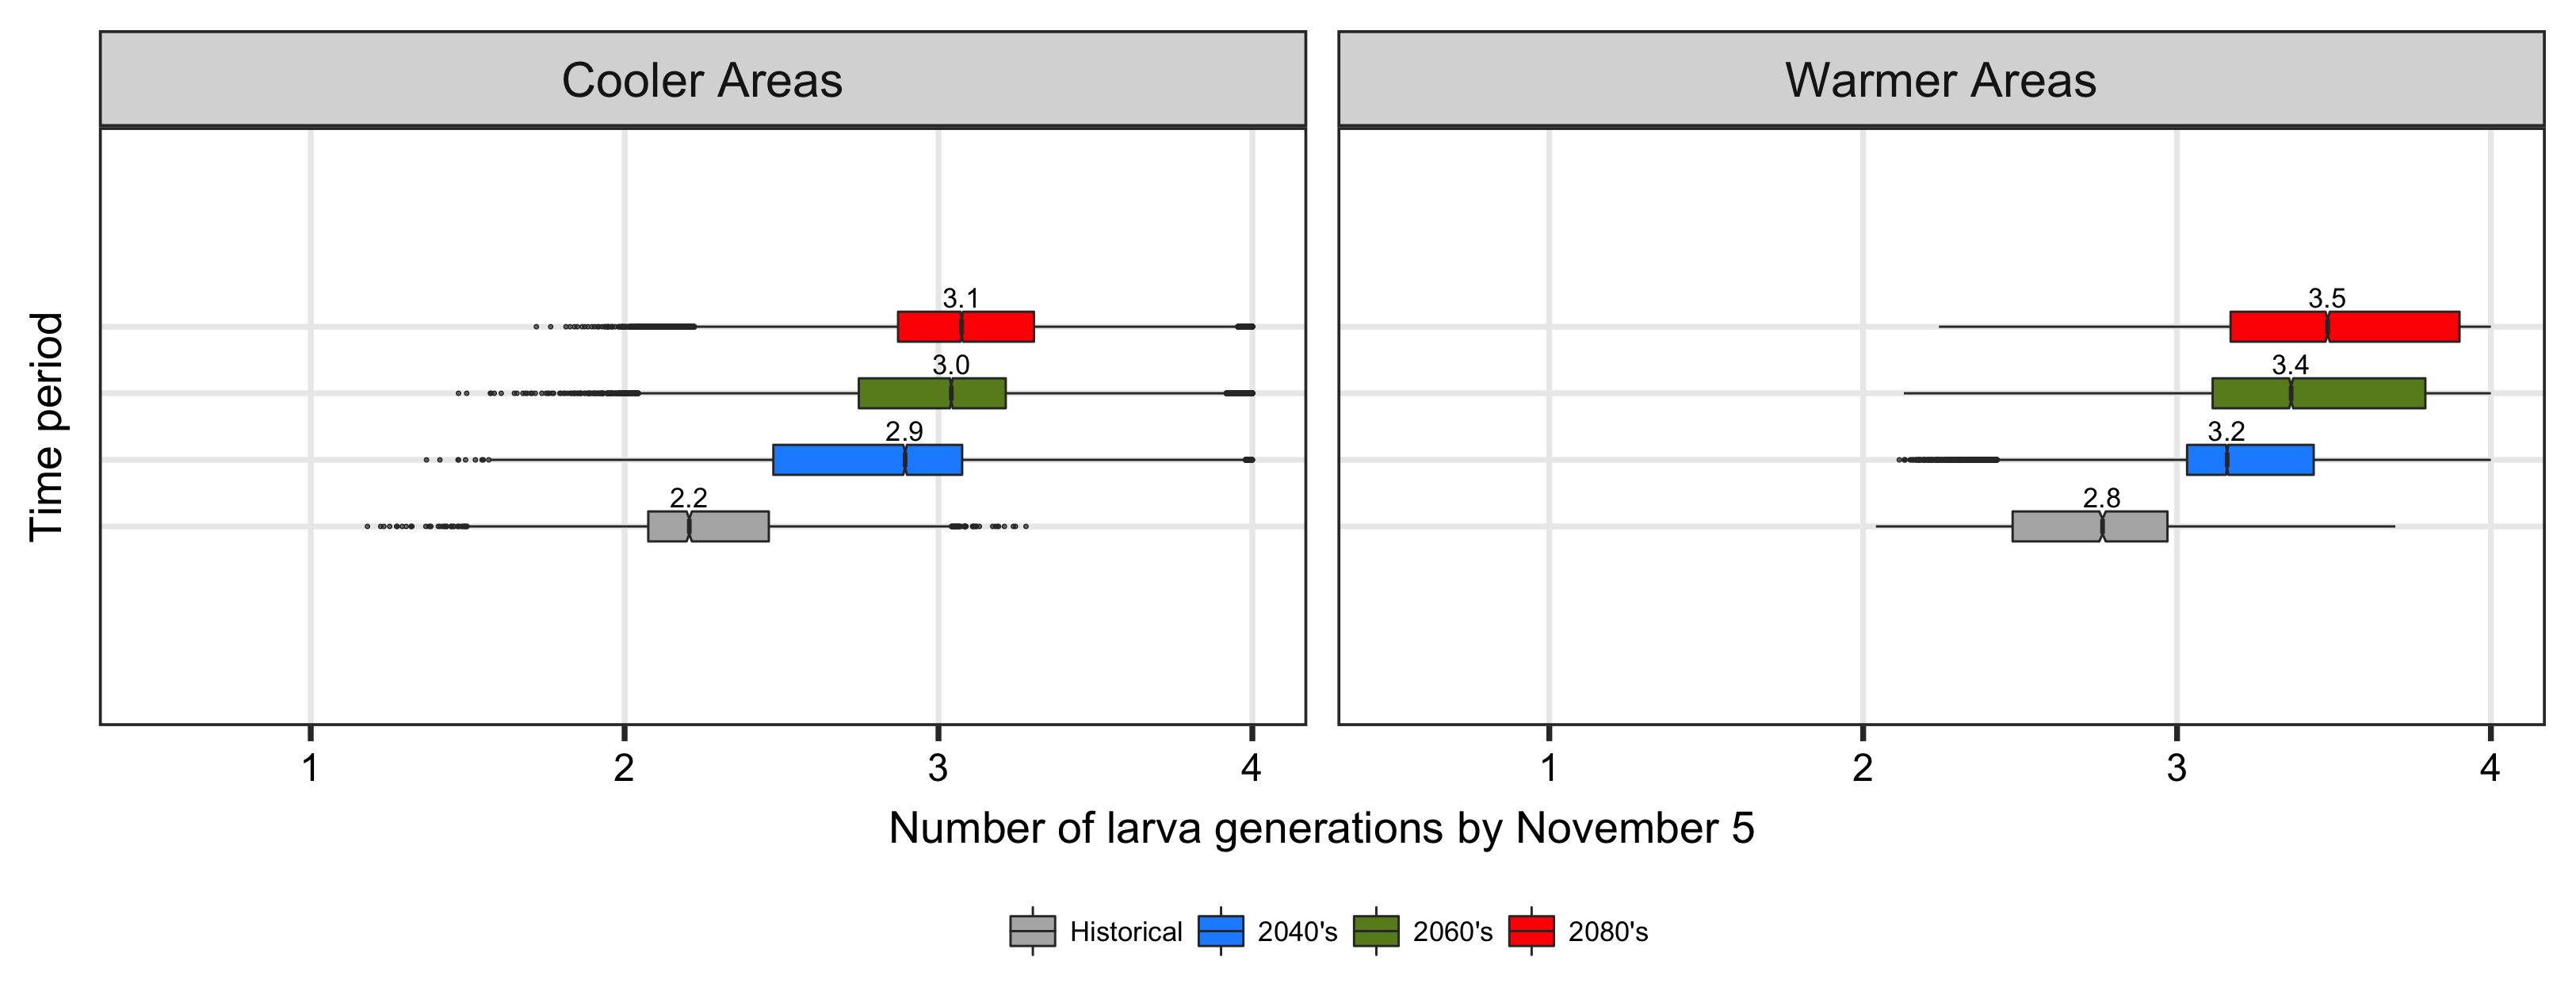
\includegraphics[width=\textwidth]{figures/Larva_Gen_Nov_rcp45}
    \end{subfigure}
     %add desired spacing between images, e. g. ~, \quad, \qquad, \hfill etc. 
      %(or a blank line to force the subfigure onto a new line)
    \begin{subfigure}[b]{0.45\textwidth}
        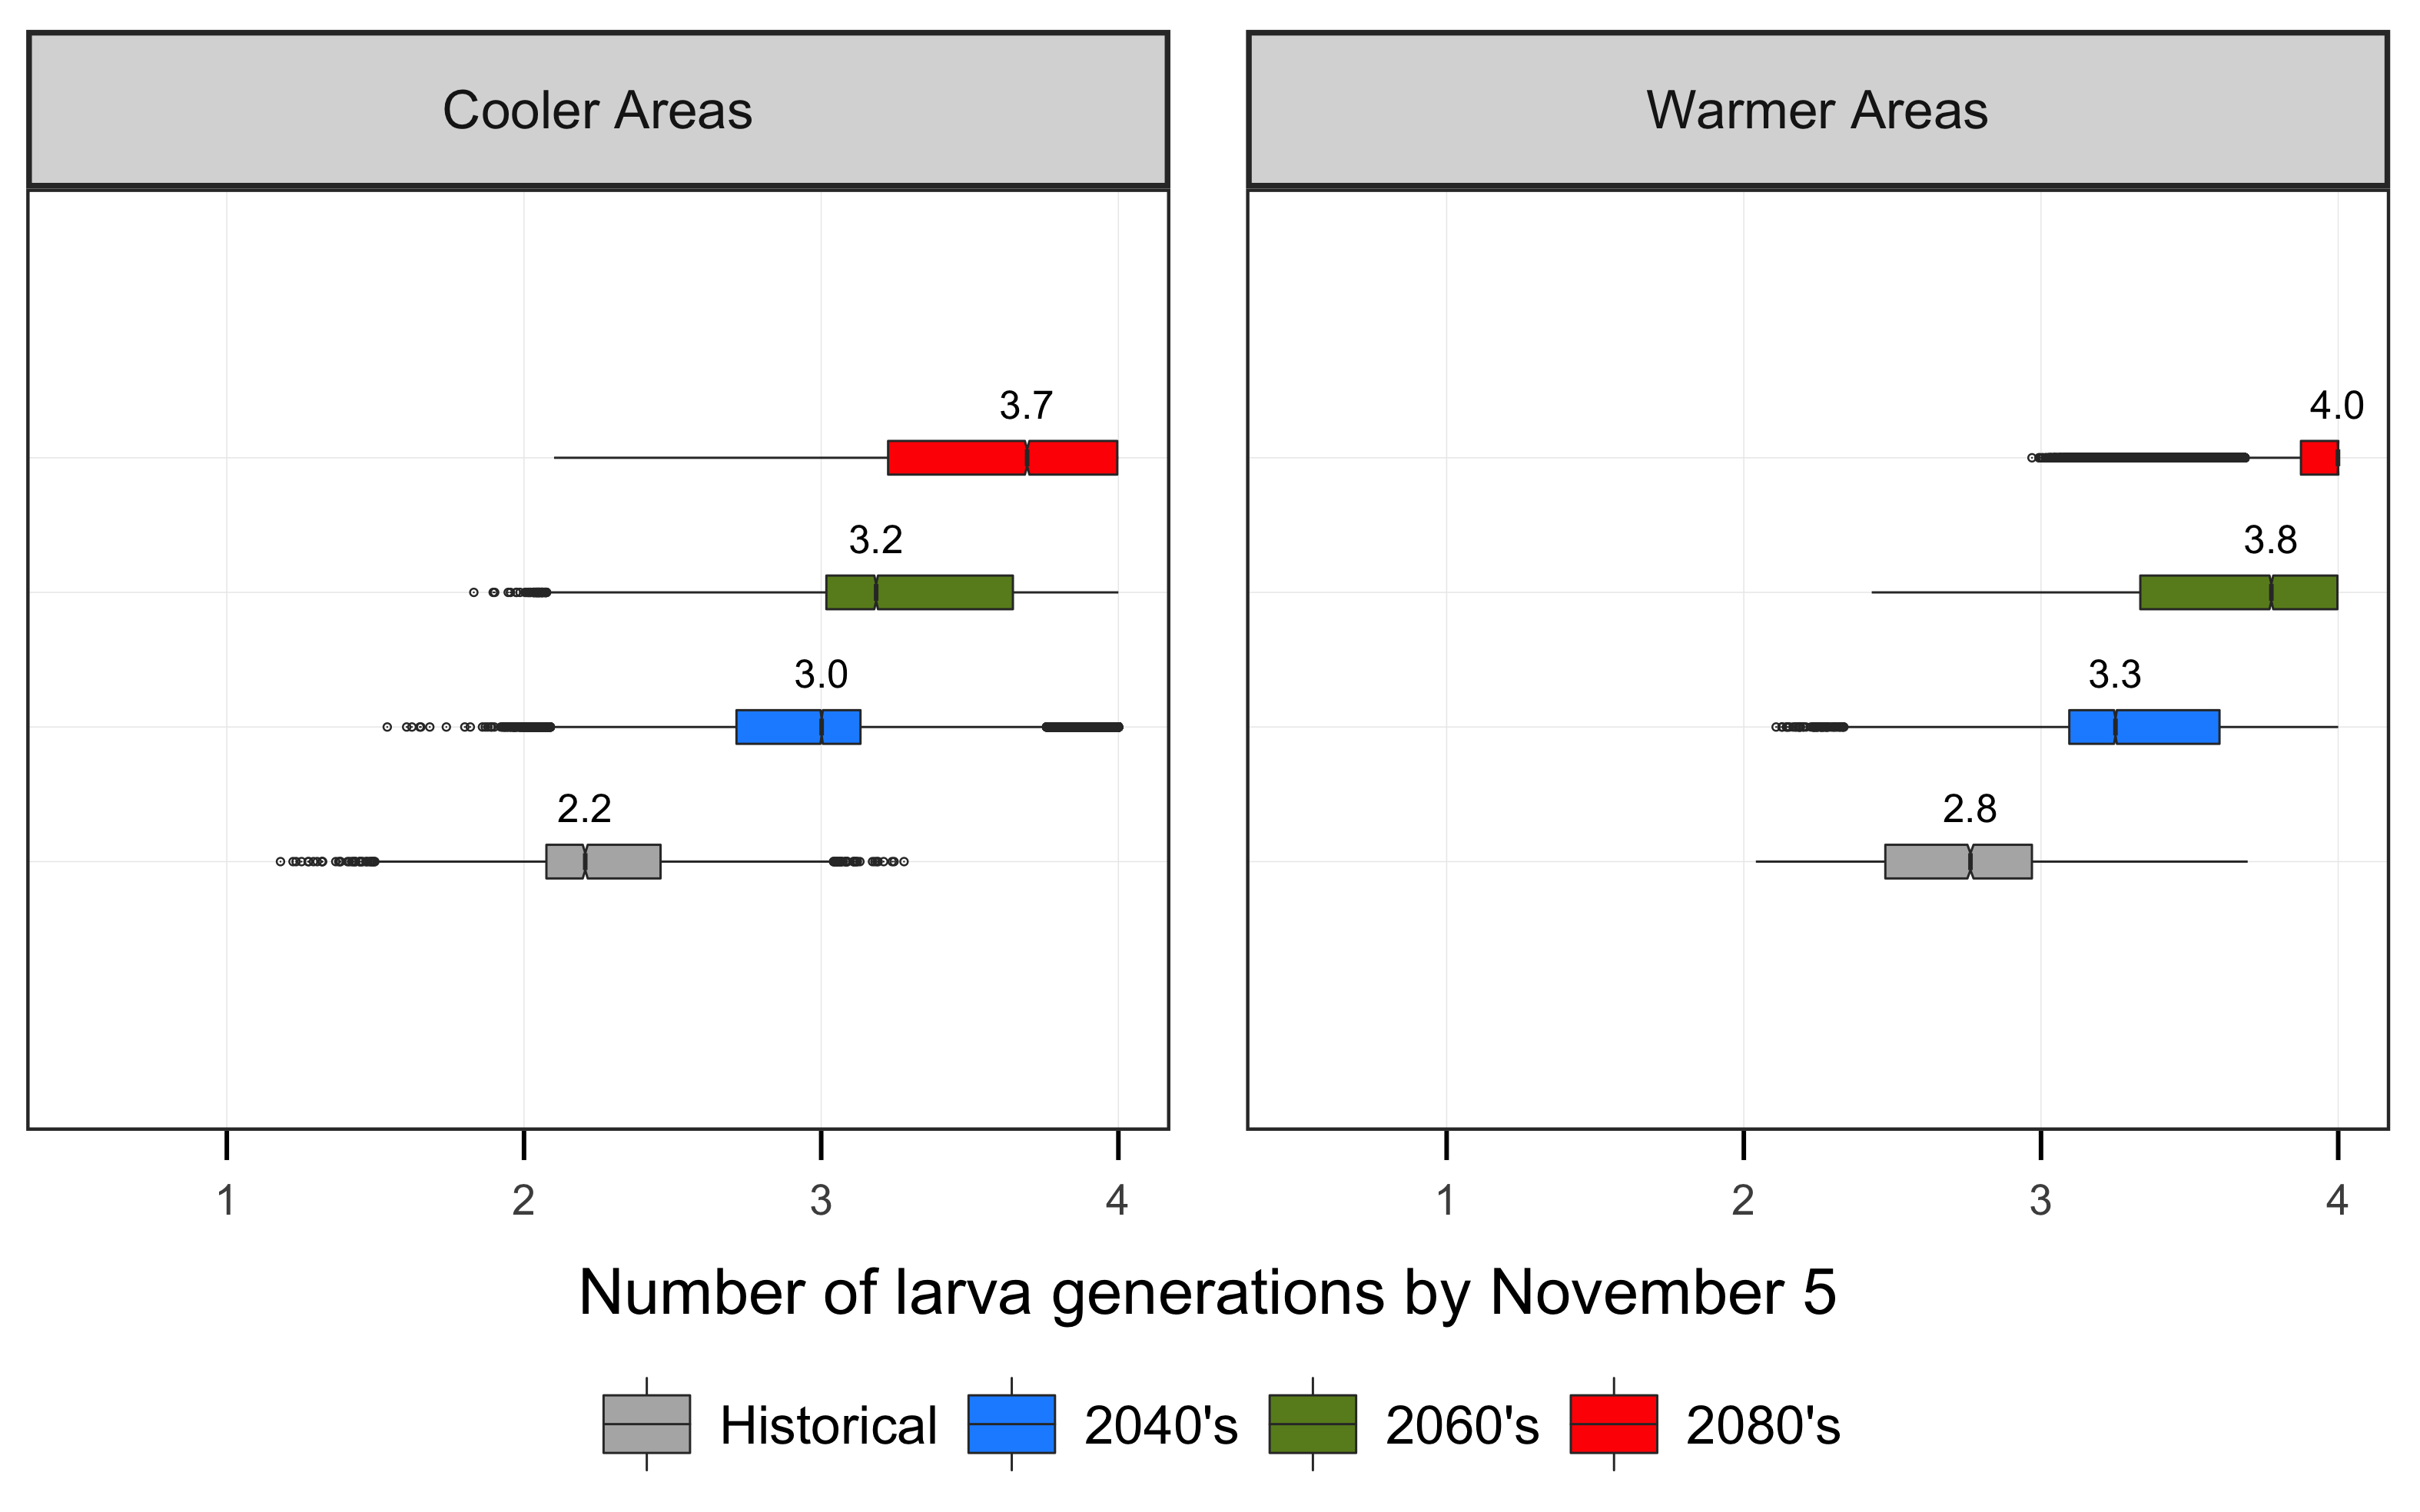
\includegraphics[width=\textwidth]{figures/Larva_Gen_Nov_rcp85}
    \end{subfigure}\\
    \caption{Changes in the number of generations of the pest}\label{fig:CNGP}
\end{figure}

\pagebreak
%%%%%%%%%%%%%%%%%%%%%%%%%%%%%%%%%%%%%%%%%%%%%%%%%
%%%%%%%%%%%%%%%%%%%%%%%%%%%%%%%%%%%%%%%%%%%%%%%%%


\subsection{Relative fraction of larvae escaping diapause induction}
Some text has to go here.
\begin{figure}[h!]
    \centering
    \begin{subfigure}[b]{0.45\textwidth}
        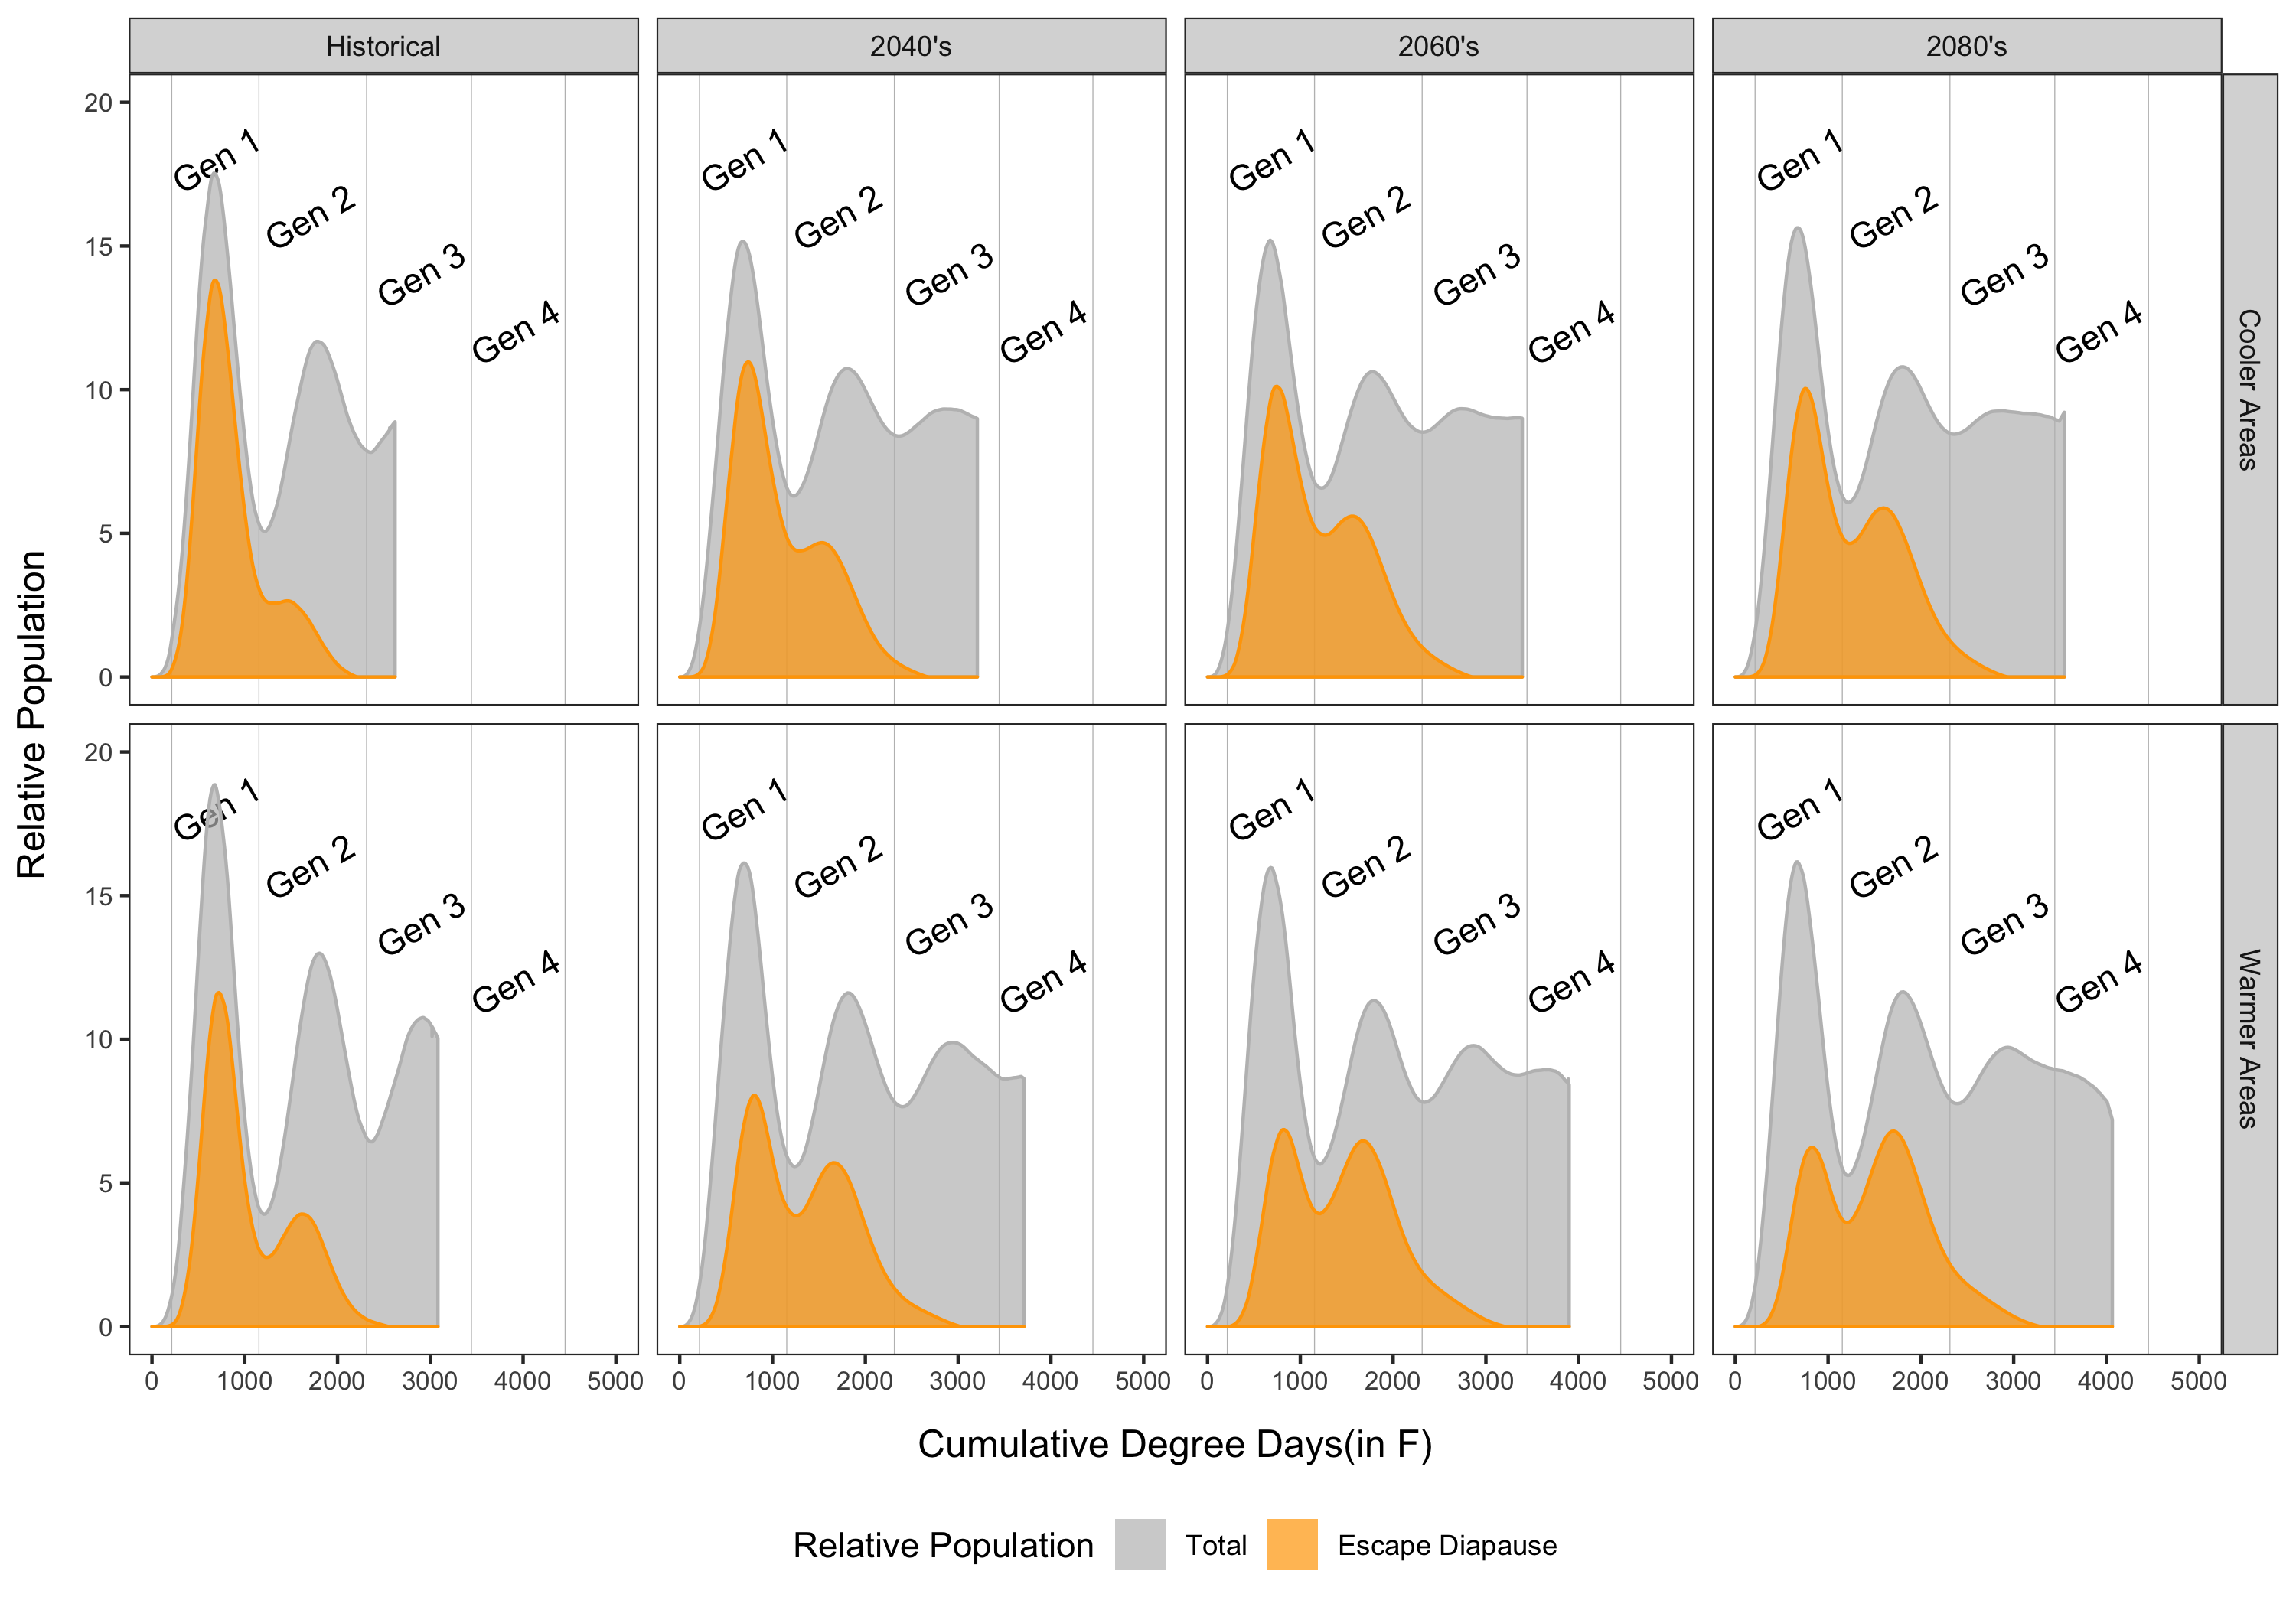
\includegraphics[width=\textwidth]{figures/diapause_rel_rcp45}
        \caption{\scriptsize  Relative fraction of escaped larvae (rcp 4.5)}
        \label{fig:RFED_45)}
    \end{subfigure}
    ~ %add desired spacing between images, e. g. ~, \quad, \qquad, \hfill etc. 
      %(or a blank line to force the subfigure onto a new line)
    \begin{subfigure}[b]{0.45\textwidth}
        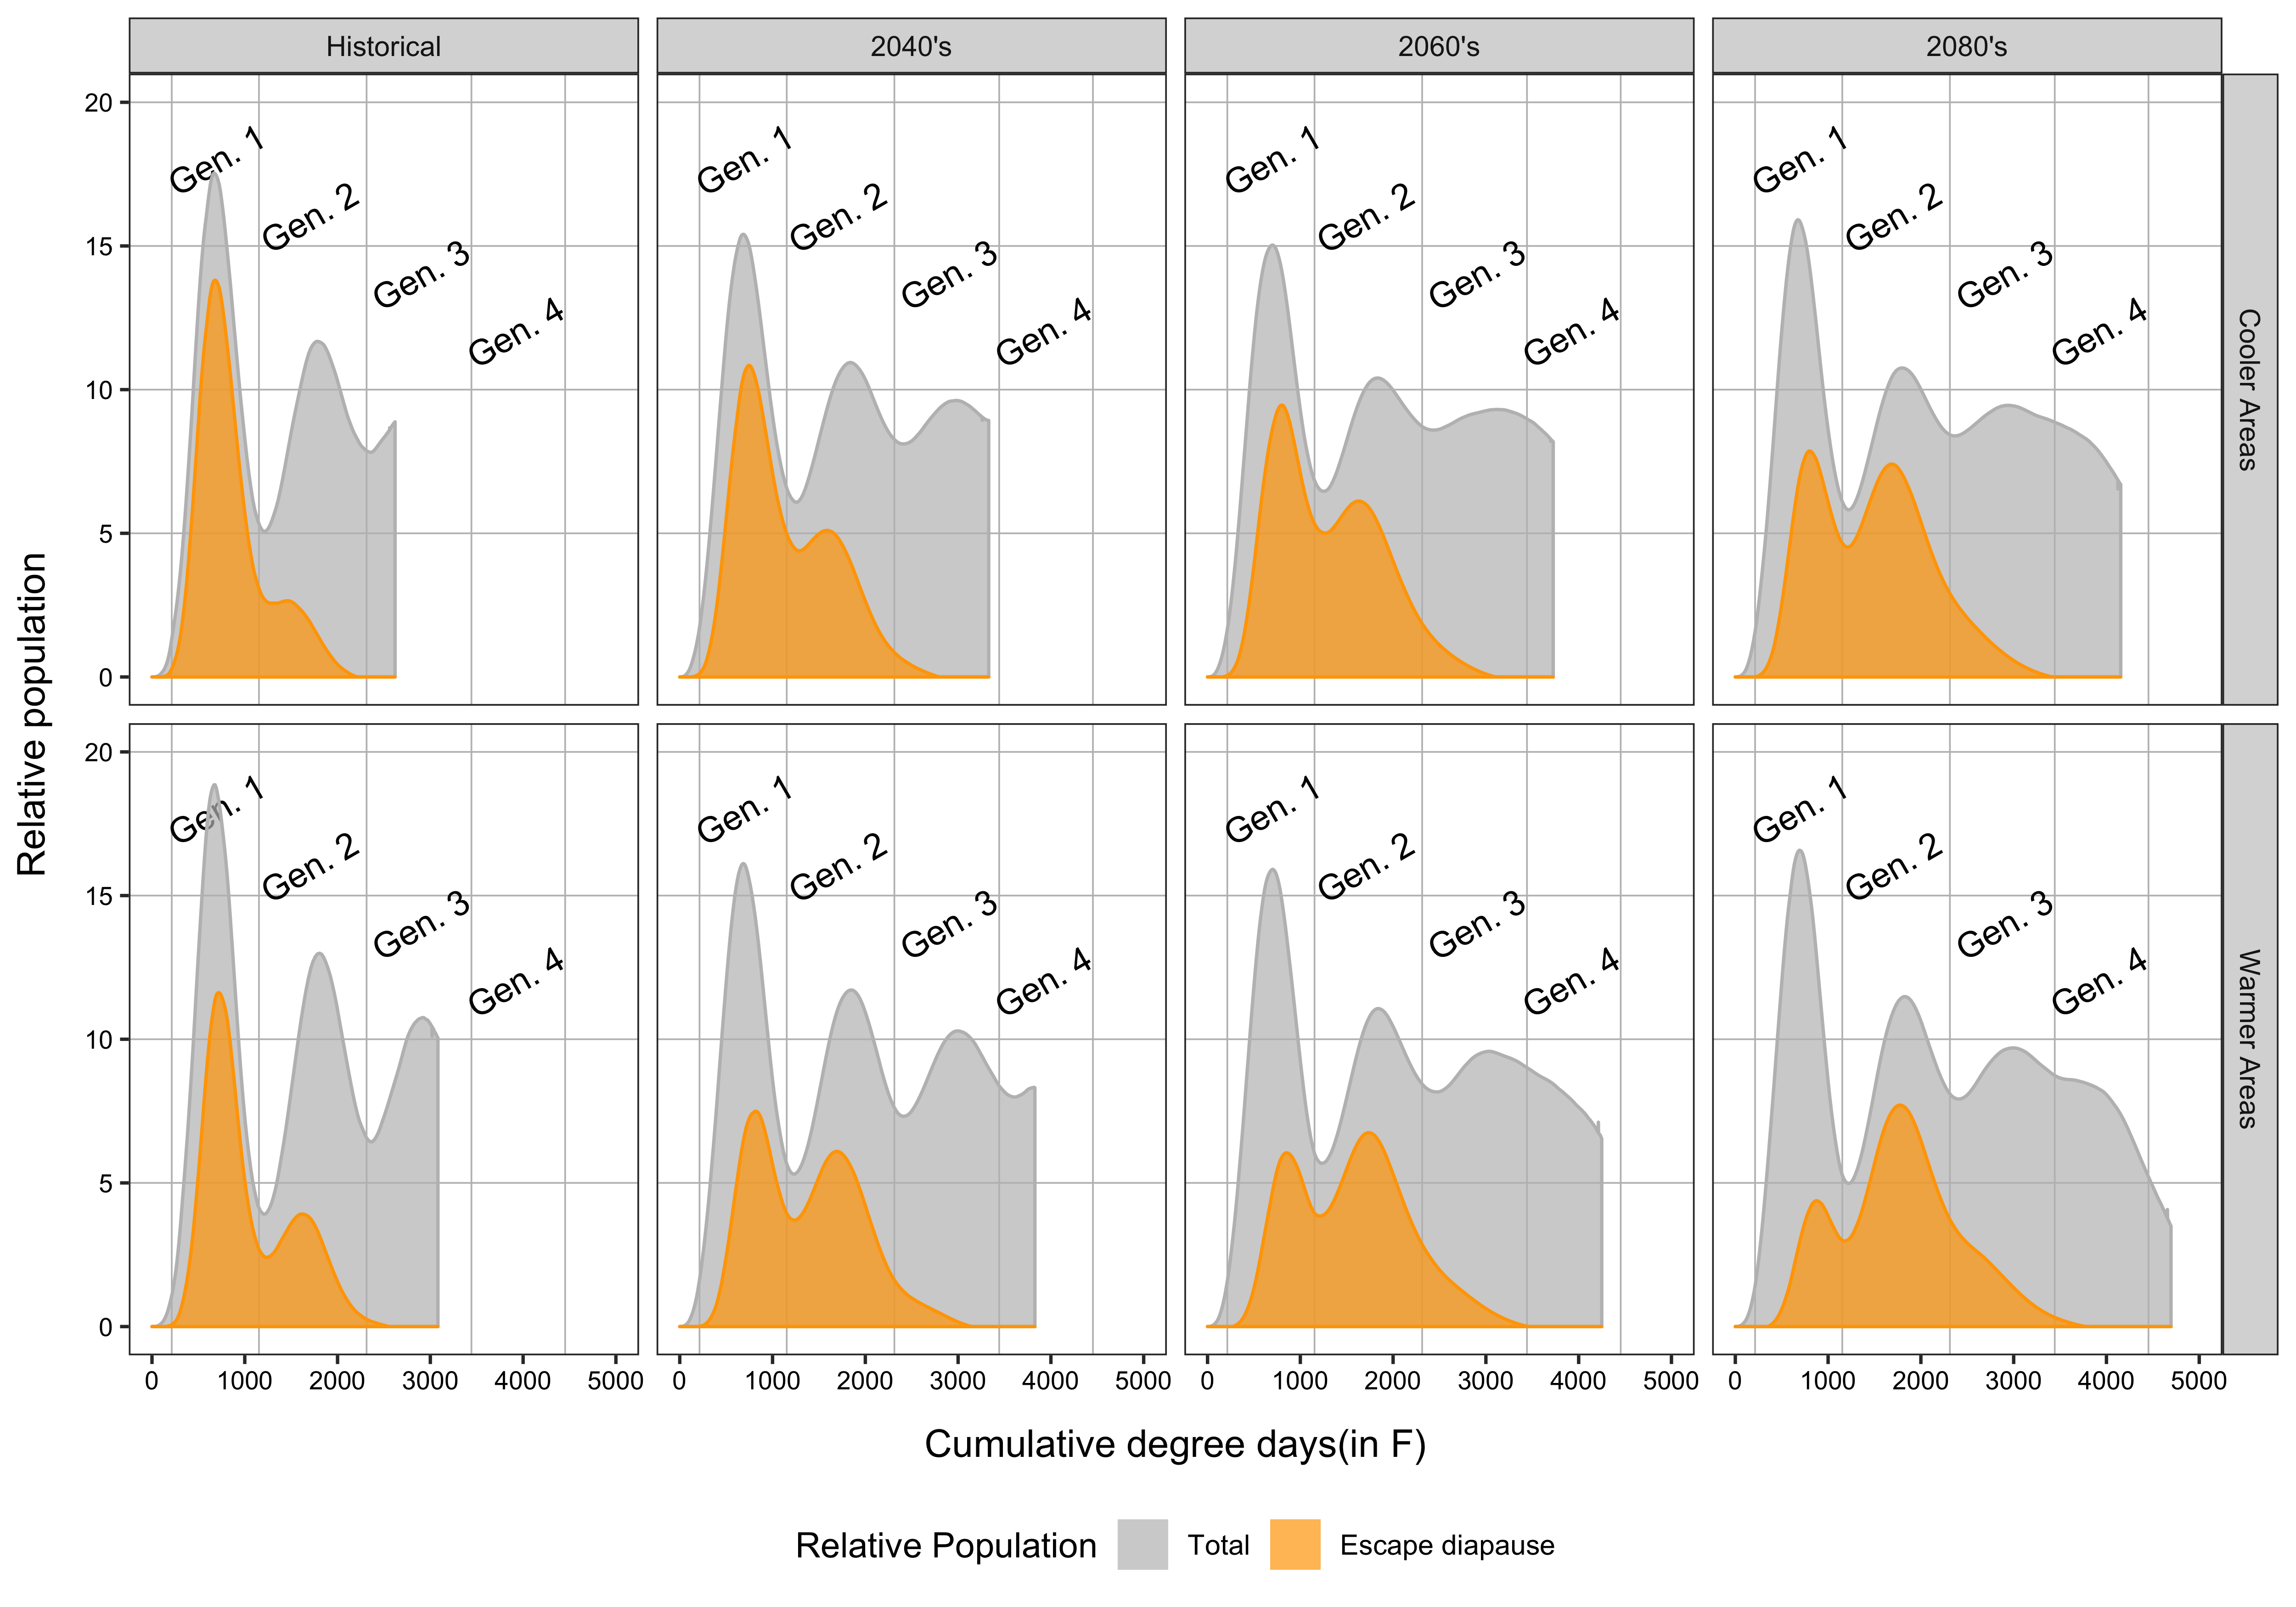
\includegraphics[width=\textwidth]{figures/diapause_rel_rcp85}
        \caption{\scriptsize Relative fraction of escaped larvae (rcp 8.5)}
        \label{fig:RFED_85}
    \end{subfigure}
    \caption{Relative fraction of larvae escaping diapause induction}\label{fig:RFLEDI}
\end{figure}



\subsection{Changes in potential for successful overwintering  (need to create)}

\subsection{Changes in the window of opportunity for pest control  (need to create)}
Create bar plots related to the  number of calendar days it takes for specific growth stages and show that it is reducing.


\subsection{Effectiveness of pest control alternatives  (Kirti to check with Vince)}
Figures similar to the new ones Vince created comparing “No control”, “Spray only”, “Spray plus Mating Disruption”


\subsection{Spatial variability in results}
Select a few maps


\subsection{Sensitivity analysis to moderations by indirect $CO_2$ effects?}
Can add diapause to photoperiod sensitivity as well if needed?
For a few select grids. (Added this section based on some lit review I found and added to the discussion section.)

\section{Discussion (Kirti, Vince)}

The timing of all codling moth growth stages shift to 
earlier in the year. In addition, a reduced time to complete 
each growth stage and longer season of higher temperatures 
both allow for a higher number of generations of the 
codling moth. This increased pest pressure is consistent 
with results focused on other parts of the United States 
and world~\cite{Juszczak2013, Rafoss_Trond, Stoeckli_2012} (Luedeling et al., 2011). 
This potentially implies the need for additional 
pesticide sprays and larger range of chemicals, 
which translates to increased cost of pest control. 
It also implies increased pesticide resistance risks. 
Given shifts in the relative fraction of larvae escaping 
diapause induction, the second generation of the codling 
moth is likely to be larger problem than has been in 
the past, and require more control.


There is limited discussion in the literature of 
potential management implications as a result 
of changing pest pressures due to warming. With 
accelerated completion of growth stages, the window 
of opportunity for pest control is reduced. Therefore 
if the ideal spray timing is missed even by a day, 
a larger number of codling moth escape control 
and cause damage. This underscores the importance 
of weather-based decision support products to 
forecast spray timing. On the flip side, if the timing 
is captured right, control mechanisms can be more 
effective under warming. For a given pesticide 
residual time or mating delay, a larger proportion 
of pests pass through susceptible growth stages 
and can be controlled. Although there is potential 
for more pest generations under warming, if the 
first generation of the pest is effectively controlled, 
the risk of damage from additional generations is 
minimal. A control program solely based on pesticides 
is not as effective and it is critical to include non-pesticide 
control mechanisms such as mating disruption in the 
mix. Something about mating disruption not being 
as sensitive to getting the application timing right 
because they have longer residual lives?  
California is already using...The longer season 
length might require availability of pheromone 
products that have a longer residual life than 
currently available. ***This section needs to be corrected and expanded.****

Multiple factors outside of what has been 
considered in this work can affect pest 
pressures and management implications 
under warming. Shifts in tree fruit phenology 
(harvest timing), and its intersection with shifts 
in insect phenology can have implications in 
terms of availability of food for larvae. Earlier 
fruit maturity under accelerated growing degree 
day accumulation, and resulting lack/unavailability
 of food for larvae could/can constrain development of 
 additional pest generations postharvest. In this case, 
 our pest pressure results would be an overestimate. 
 However, from a practical orchard management 
 perspective, apples left on the ground 
 postharvest can act as a food source for 
 CM larvae. Also increased pest pressures 
 in backyard gardens - which are not well 
 managed in comparison to commercial orchards 
 - will continue to be an issue for commercial 
 orchards bordering urban boundaries. 
 Additionally, accelerated maturity in crops is 
 typically associated with decreases in yields~\cite{Rajagopalan_Chin}
, and as an 
 adaptation response to address yield decreases, 
 crop breeding technologies may provide slower 
 maturing crop varieties. So food availability 
 may not necessarily moderate potential 
 increases in pest pressures to the extent expected.
 
 Our results do not consider the effect of 
 elevated CO2 levels on CM pressures 
 and management because there are no 
 critical direct effects on insect physiology 
 and phenology~\cite{Patterson1999}. 
 However, elevated CO2 levels have a direct 
 effect on the pest’s host plant~\cite{Patterson1999} 
 by increasing the carbon to nitrogen ratio 
 (less relative nitrogen which is a limiting factor 
 for insect performance), and therefore there are 
 potential indirect effects for pests: larvae need 
 to eat more, delayed larval growth~\cite{Stiling_1823}, 
 and elevated 
 mortality rates to stressors such as heat~\cite{Lindroth_1996}. 
 By not considering these 
 indirect effects, we may be overestimating pest pressures.

Empirical models designed for historical conditions 
are extrapolated into the future. This assumes a 
continued linear response of insect phenology and 
physiology to elevated temperatures, while temperature 
responses are often non-linear and empirical models 
likely need adjustment to better represent responses 
to conditions outside of what they they were developed 
for~\cite{Andrea_Maiorano} (Luedeling et al., 2011). 
Non-linearity and increased mortality of high temperatures, 
likely implies that pest pressures are overestimated. 
However, there is also experimental evidence that the 
codling moth has demonstrated ability to adjust to 
high temperatures~\cite{Frank_Rapid}. 
Should we add some discussion of upper thresholds 
of the model, how often we exceed them etc., to show the 
model seems relevant until we go well into the future. 

Based on field experiments at a limited number 
of locations for a limited number years, our model 
for the codling moth’s diapause induction in 
Washington state is a function of just the photoperiod. 
In Mexico - at a lower latitude with higher average 
temperatures than Washington state - diapause 
induction has been modeled as a photothermic 
response~\cite{Cuellar_2005}, where 
it is dependent of photoperiod and temperature. 
The magnitude of pest pressure changes is highly 
sensitive to assumptions related to diapause induction 
~\cite{Stoeckli_2012}, and there is very little we 
know about this aspect. Other studies related to 
impacts of climate change on codling moth pest 
pressures have either not considered the diapause 
induction aspect~\cite{Juszczak2013} (Luedeling et al., 2011), 
or assumed that diapause induction will evolve as a 
response to climate change~\cite{Stoeckli_2012}. 
Given that …..Vince to add something about why 
we believe this evolution does not seem likely in 
the time frames we are interested in…. , we extend 
our historical diapause induction model into 
the future. However, this is a critical aspect of 
uncertainty in characterizing impacts of climate 
change to the codling moth and pests in general.

Warmer winter, mortality in field. Higher 
survival in overwintering. Insufficient chilling 
unit distort time. Not synchronised emergence 
and spread out more. Male versus female effects. 
Effective numbers of males versus females are 
not synchronised. Males tend to come out early.  Higher overwintering generations.
%%%%%%%%%%%%%%%%%%%%%%%%%%%%%%%%%%%%%%%%%%%%%%%%%
%%%%%%%%%%%%%%%%%%%%%%%%%%%%%%%%%%%%%%%%%%%%%%%%%
\section{Conclusions (Vince, Kirti)}

Consistent with other related work, there are 
signs of increased codling moth pressures under 
higher future temperature projections. However, it 
is likely that transformational changes in management
 would not be necessary. Multiple factors 
 contribute to this. First, the first generation 
 population that escapes diapause induction 
 is likely lower, and if this first generation pest 
 is controlled well, future increased potential 
 number of generations are less of an issue. 
 Second, if timed right, control mechanisms 
 such as pesticides and mating disruption tend 
 to be more effective under warmer temperatures. 
 Third there is potential for a higher mortality rate 
 under warming; however, the codling moth has 
 shown strong adaptive capacity to this in 
 experiments, and it may not be a moderating 
 factor. Fourth, other factors such as indirect effect 
 of elevated CO2 levels moderate temperature 
 related increases in pest pressures, through delayed 
 pest development. Although delayed development 
 of pest reduces pest pressure in terms of the 
 potential number generations of pest, it also
  potentially  negates increases in effectiveness 
  of pest control mechanisms.  Knowledge gaps 
  related to our understanding of pest response 
  to warming - such as diapause induction, 
  non-linearity in pest response to temperatures
   beyond the historical range, and pest/host 
   interactions - lead to uncertainty in future projects 
   of codling moth management. Many of the 
   responses are competing in nature and negate 
   each other. Therefore, while climate change 
   impacts on codling moth pest pressures are 
   largely negative when temperature effects 
   are considered in isolation, multiple factors 
   point to the possibility of a less severe net 
   effect of climate change on codling moth 
   pest pressures,  and pest management 
   unlikely to need major transformative changes.
%%%%%%%%%%%%%%%%%%%%%%%%%%%%%%%%%%%%%%%%%%%%%%%%%
%%%%%%%%%%%%%%%%%%%%%%%%%%%%%%%%%%%%%%%%%%%%%%%%%
\section{Figures and Tables (Min, Giridhar)}

%%%%%%%%%%%%%%%%%%%%%%%%%%%%%%%%%%%%%%%%%%%%%%%%%
%%%%%%%%%%%%%%%%%%%%%%%%%%%%%%%%%%%%%%%%%%%%%%%%%
\section{Kirti’s compiled list of potential references and summary notes}
(Harrington et al., 2001) Discusses the question: Can 
climate change impacts on insects be predicted?  
Notes that with climate change there are implications 
for effectiveness of pest control mechanisms as well. 
This is however  not discussed in the way we do it. More 
in terms of dryer future implying more suitable days for 
spraying. Can use as reference for noting implications 
for effectiveness of pest control measures.
(Fleming \& Tatchell, 1995) and (Zhou et al., 1996)  

There is evidence for impacts in historical records as 
well. Historical long term records of aphids and 
advancement in phenology of 10 days over a period 
of 21 year for across several latitudes.

(Stoeckli et al., 2012)~\cite{Stoeckli} climate change impacts in a 
few regions in Switzerland. Assumes there will be 
adaptation in photoperiod requirements for diapause
 induction and does a sensitivity analysis. No 
 detailed discussions on management implications.
(Chidawanyika \& Terblanche, 2011) We do not 
consider mortality rate under elevated temperatures. 
Can this be used as evidence that CM has 
demonstrated ability to adjust to it?
(Luedeling et al., 2011) CM in Walnuts in 
California ( currently 2 to 4 generations) 
Well written paper.

(Steinberg et al., 1988) Higher pre-diapause 
temperatures caused earlier diapause induction. 
Immature fruit delayed diapause induction. 
(Jacobo-Cuellar et al., 2005) Diapause induction 
as a function of photoperiod and temperature.
(Maiorano et al., 2012) Discusses the fact that 
empirical models assume linear temp responses 
to continue in the same way, while in reality the 
responses are typically non-linear and level off. 
There is the heat stress aspect as well. So it 
may be not be appropriate to extrapolate these 
into the future. Perhaps briefly mention this as 
a potential limitation. We can reference 
Luedling et al. 2011 as well.
(Patterson et al., 1999) Climate-change 
weeds, insects…...

(Cossentine et al., 2004) Discusses something 
about CO2 in relation to fumigation of apple 
packing boxes. Don’t think this is  is applicable, 
but adding it just in case.
(Gregory et al., 2009) Importance of integrating 
pests into the climate change/food security 
debate. Has useful references we could add.
(Zvereva \& Kozlov, 2006; Stiling \& Cornelissen, 2007)  
Zvereva Elevated Temp positively affects 
insect performance while Co2 negatively 
effects and when considering them 
simultaneous the effects are negated. 
Stiling note that under elevated CO2 
there were considerable reductions in 
leaf miner consumption rate, total 
consumption, development rate etc.


\bibliographystyle{plain}
\bibliography{cod_moth_bib}

\end{document}
